\documentclass[a4paper,12pt]{report}

\usepackage{styles/report_format}

% for bibliography
\usepackage[style=ieee]{biblatex}
\addbibresource{references.bib}

\RequirePackage{fix-cm}
\usepackage{fontspec}
\setmainfont{Times New Roman}

\usepackage{graphicx}
\usepackage{amsmath, amssymb}
\usepackage{longtable}
\usepackage{algorithm}
\usepackage{algorithmic}
\usepackage{hyperref}
\usepackage{placeins}
\usepackage{enumitem}
\usepackage{xcolor}
\usepackage{makecell}
\usepackage{array}

% Directory of figures
\graphicspath{{figures/}}

% Times New Roman, Requires XeLaTeX or LuaLaTeX
\RequirePackage{fix-cm}
\usepackage{fontspec}
\setmainfont{Times New Roman}


% Numbering at bottom
\usepackage{fancyhdr}
\pagestyle{fancy}
\fancyhf{}% Clear page header/footer
\renewcommand{\headrulewidth}{0pt}% No header rule
\fancyfoot[C]{\thepage}

% Page Margins
\usepackage[top=3.5cm,bottom=2cm,left=3.5cm,right=2cm]{geometry}

% COVER PAGE INFO
\title{BINARY NEURAL NETWORK IMPLEMENTATION FOR HANDWRITTEN DIGIT RECOGNITION ON FPGA}
\turkcebaslik{FPGA ÜZERİNDE EL YAZISI RAKAM TANIMA İÇİN BİNARY NÖRAL AĞ UYGULAMASI}
\author{Emir Devlet Ertörer}
\subyear{2025}

% APPROVAL PAGE INFO
\supervisor{Prof. Cem Ünsalan}
\examineri{(Examiner 1 Name)}
\examinerii{(Examiner 2 Name)}
\dateofapproval{.../.../2025}

\begin{document}
\pagenumbering{roman}

% COVER PAGE
\makecoverpage

% BLANK PAGE
\clearpage\mbox{}\clearpage\addtocounter{page}{-1}

% APPROVAL PAGE
\makeapprovalpage

% ACKNOWLEDGEMENTS
\begin{acknowledgements}

\end{acknowledgements}

% ABSTRACT
\begin{abstract}
Image recognition has gained significant importance over the past decades, with neural network models widely deployed across a range of applications. While traditional deep learning models achieve high accuracy, they often require substantial computational resources and memory. Binary Neural Networks (BNNs) present a highly efficient alternative by reducing both the size and complexity of the model, making them especially suitable for deployment on resource constrained platforms. Due to their binarized weights and activations, BNNs can achieve faster inference and lower power consumption compared to full precision models. This project focuses on the implementation of a trained BNN for handwritten digit recognition and its deployment on a Field Programmable Gate Array (FPGA). The design leverages the parallel processing capabilities of FPGAs to achieve real-time inference while maintaining a compact hardware. 

\end{abstract}

% ÖZET
\begin{ozet}
Görüntü tanıma, son yıllarda önemli bir gelişme göstermiş ve sinir ağı modelleri birçok alanda yaygın şekilde kullanılmaya başlanmıştır. Geleneksel derin öğrenme modelleri yüksek doğruluk oranlarına ulaşsa da, genellikle yüksek hesaplama gücü ve bellek gereksinimi duyarlar. Binary Neural Network (BNN) modelleri ise, modelin boyutunu ve karmaşıklığını azaltarak özellikle donanım kaynakları sınırlı olan sistemler için oldukça verimli bir alternatif sunar. Ağırlıkların ve aktivasyonların binarize edilmesi sayesinde BNN’ler, tam hassasiyetli modellere kıyasla daha hızlı çıkarım (inference) yapabilirler ve daha az güç tüketirler. Bu proje, el yazısı rakamların tanınması için eğitilmiş bir BNN modelinin Field Programmable Gate Array (FPGA) üzerinde uygulanmasına odaklanmaktadır. Tasarım, FPGA’nin paralel işlem yeteneklerinden faydalanarak gerçek zamanlı çıkarım sağlamayı hedeflemekte ve donanımın kompakt yapısını korumaktadır.

\end{ozet}

% TABLE OF CONTENTS, LISTS
\tableofcontents

\listoffigures

\listoftables

% ABBREVIATIONS
\begin{symbols-abbreviations}
\sym{FPGA}{Field Programmable Gate Array}
\sym{BNN}{Binary Neural Network}
\sym{CLB}{Configurable Logic Block}
\sym{LUT}{Look-Up Table}
\sym{CNN}{Convolutional Neural Network}
\sym{CPU}{Central Processing Unit}
\sym{GPU}{Graphics Processing Unit}
\sym{ReLU}{Rectified Linear Unit}
\sym{STE}{Straight-Through Estimator}
\sym{XNOR}{Exclusive NOR (bitwise operation)}
\sym{SBN}{Shift-based Batch Normalization}
\sym{AdaMax}{Adaptive Moment Estimation Max Optimizer}
\sym{QAT}{Quantization Aware Training}
\sym{HLS}{High Level Synthesis}
\end{symbols-abbreviations}



% CHAPTER 1 - INTRODUCTION
% -------------------------
\clearpage
\chapter{INTRODUCTION}
\label{chapter:introduction}
\pagenumbering{arabic}


\section{Binarized Neural Networks (BNNs)}
The continuous progress in the field of deep learning \cite{lecun2015deep} has led to major advancements in areas such as speech recognition, generative AI, large language models and computer vision. Among the most widely used architectures are Convolutional Neural Networks (CNNs), which owe their popularity to their deep structure and large number of parameters, often ranging from millions to billions. These models have achieved state-of-the-art performance across a wide range of tasks.

Despite their high accuracy, CNNs rely heavily on precise floating-point computations, typically using 32-bit representations. This leads to significant computational and memory usage. As a result, deploying CNN models typically requires high performance hardware, such as modern Graphics Processing Units (GPUs) or specialized Central Processing Units (CPUs).

Research has shown that CNNs include large redundancies in their structure \cite{6797077}. This has led to the development of various model compression techniques that try to reduce the memory and computational resource usage without severely impacting performance and accuracy. One of the most effective compression techniques is quantization, where weights and activations are represented using low-precision numbers. Within this category, binary quantization is the most aggressive form of quantization. It restricts weights and activations to just two possible values: -1 and +1 (or 0 and 1).

This form of quantization results in a special class of models known as Binary Neural Networks (BNNs). By representing both weights and activations using only 1 bit instead of 32 bits, BNNs drastically reduce memory usage. Additionally, expensive floating-point matrix multiplications can be replaced with lightweight bitwise operations, such as the XNOR and bitcount, which offer significant speedup. For instance, BNNs can achieve up to 32× memory savings and up to 58× computational speedup on CPUs \cite[p.~4]{Qin_2020}.

Due to their lightweight and efficient structure, BNNs are particularly well suited for deployment on embedded and resource constrained platforms, such as FPGAs and mobile devices \cite{Qin_2020}.


\subsection{Forward Propagation in BNNs}
To understand how forward propagation works in BNNs, it is helpful to first understand how standard neural networks work. In any neural network, each layer contains a set of \textit{weights} (learnable parameters) that determine how much influence each input has on the output of a neuron. These weights are initially assigned random values and are updated through training so that the network can learn patterns from the provided data.

During forward propagation, each neuron receives a set of input values (called \textit{activations}) and computes a weighted sum of these inputs:
\[z = \sum_{i=1}^{n} w_i \cdot x_i\]
This value \(z\) is then passed through an \textit{activation function} (such as the ReLU or sigmoid function) to produce the neuron’s output. The purpose of this computation is to transform the input in a way that helps the network make correct predictions. The weighted sum captures how strongly the input features are aligned with the learned weights and the activation function determines whether the neuron should be activated based on this value. This selective activation allows the network to capture complex patterns and make distinctions between different classes or outputs.

BNNs simplify this process by constraining both the weights \(w_i\) and activations \(x_i\) to binary values, typically \( \{-1, +1\} \). This allows computationally expensive floating-point multiplications to be replaced with bitwise \textit{XNOR} operation. In binary logic, the XNOR gate outputs 1 when both inputs are the same and 0 otherwise. Therefore, if \(x_i\) and \(w_i\) are encoded as 1 for +1 and 0 for –1, then:
\[\text{XNOR}(x_i, w_i) = 
\begin{cases}
1, & x_i = w_i \\
0, & x_i \neq w_i
\end{cases}\]
Applying the XNOR operation to each element in two binary vectors \(x\) and \(w\), we obtain a new binary vector indicating which elements match. The number of 1s in the result (called the \textit{popcount}) tells us how many inputs matched their corresponding weights:
\[\text{popcount}(\text{XNOR}(x, w)) = \sum_{i=1}^n [x_i = w_i]\]
This count alone does not fully represent the dot product. In BNNs, the goal is to replicate the dot product using only bitwise operations. When \(x_i\) and \(w_i\) are equal (both \(+1\) or both \(-1\)), their product is \(+1\). When they are different, the product is \(-1\). Therefore, the number of matches contributes \(+1\) each and mismatches contribute \(-1\) each.

Let \(m\) be the number of matching elements and \(n\) the total number of elements in the vectors. The number of mismatches is then \(n - m\), and the signed dot product becomes:
\[z = (m \cdot +1) + ((n - m) \cdot -1)\]
Which can be simplified as:
\[z = m - (n - m) = 2m - n\]
Since \(m = \text{popcount}(\text{XNOR}(x, w))\), we can express the full dot product approximation as:
\[z \approx 2 \cdot \text{popcount}(\text{XNOR}(x, w)) - n\]
This transformation allows us to simulate the original full dot product between binary vectors using only XNOR and popcount operations, which are much more efficient in digital hardware than multiplications and additions.

To make this XNOR based computation possible, both the input activations and the weights must first be binarized. This is done using the \textbf{sign function}, which converts real valued inputs into binary form:
\[\text{sign}(x) = 
\begin{cases}
+1, & x \geq 0 \\
-1, & x < 0
\end{cases}\]
By applying the sign function during the forward pass, the network ensures that all computations operate on binary values. This binarization is what enables the replacement of multiplications with efficient XNOR and popcount operations.

This completes the forward pass, producing binary activations that are later compared to the true labels to compute the loss, which guides weight updates during backpropagation.


\clearpage
\subsection{Backward Propagation and the Straight-Through Estimator (STE)}
To understand how backward propagation works in BNNs, it is important to first understand the standard backpropagation algorithm used in traditional neural networks. In a conventional setting, after the forward pass computes predictions, the network calculates a loss that measures how far off the predictions are from the true labels. This loss is then propagated backward through the network using the chain rule of calculus, updating the weights to minimize future errors.

For a weight \(w\), the update is computed as:
\[w \leftarrow w - \eta \cdot \frac{\partial L}{\partial w}\]
where \( \eta \) is the learning rate and \( \frac{\partial L}{\partial w} \) is the gradient of the loss with respect to that weight. These gradients are computed by applying the chain rule through every layer of the network:
\[\frac{\partial L}{\partial w_i} = \frac{\partial L}{\partial z} \cdot \frac{\partial z}{\partial w_i}\]
Here, \(z\) is the weighted sum of inputs and \( \frac{\partial z}{\partial w_i} = x_i \) is the input to the neuron. This process works smoothly for differentiable functions like ReLU or sigmoid.

However, in Binary Neural Networks, backpropagation faces a major problem due to the use of the \textit{sign function} during binarization:
\[\text{sign}(x) = 
\begin{cases}
+1, & x \geq 0 \\
-1, & x < 0
\end{cases}\]
This function is non differentiable at \(x = 0\), and its derivative is zero almost everywhere else. As a result, the gradient \( \frac{d}{dx} \text{sign}(x) \) is either undefined or vanishes, making it impossible to propagate error signals backward. This leads to the well known \textit{vanishing gradient problem}, where gradients become too small for the network to learn effectively. In the context of BNNs, this problem is especially severe because the sign function provides no useful gradient information during backpropagation. Without intervention, the model is unable to update its parameters, effectively stopping the learning process \cite{bengio2013estimatingpropagatinggradientsstochastic}.

\begin{figure}[htbp]
    \centering
    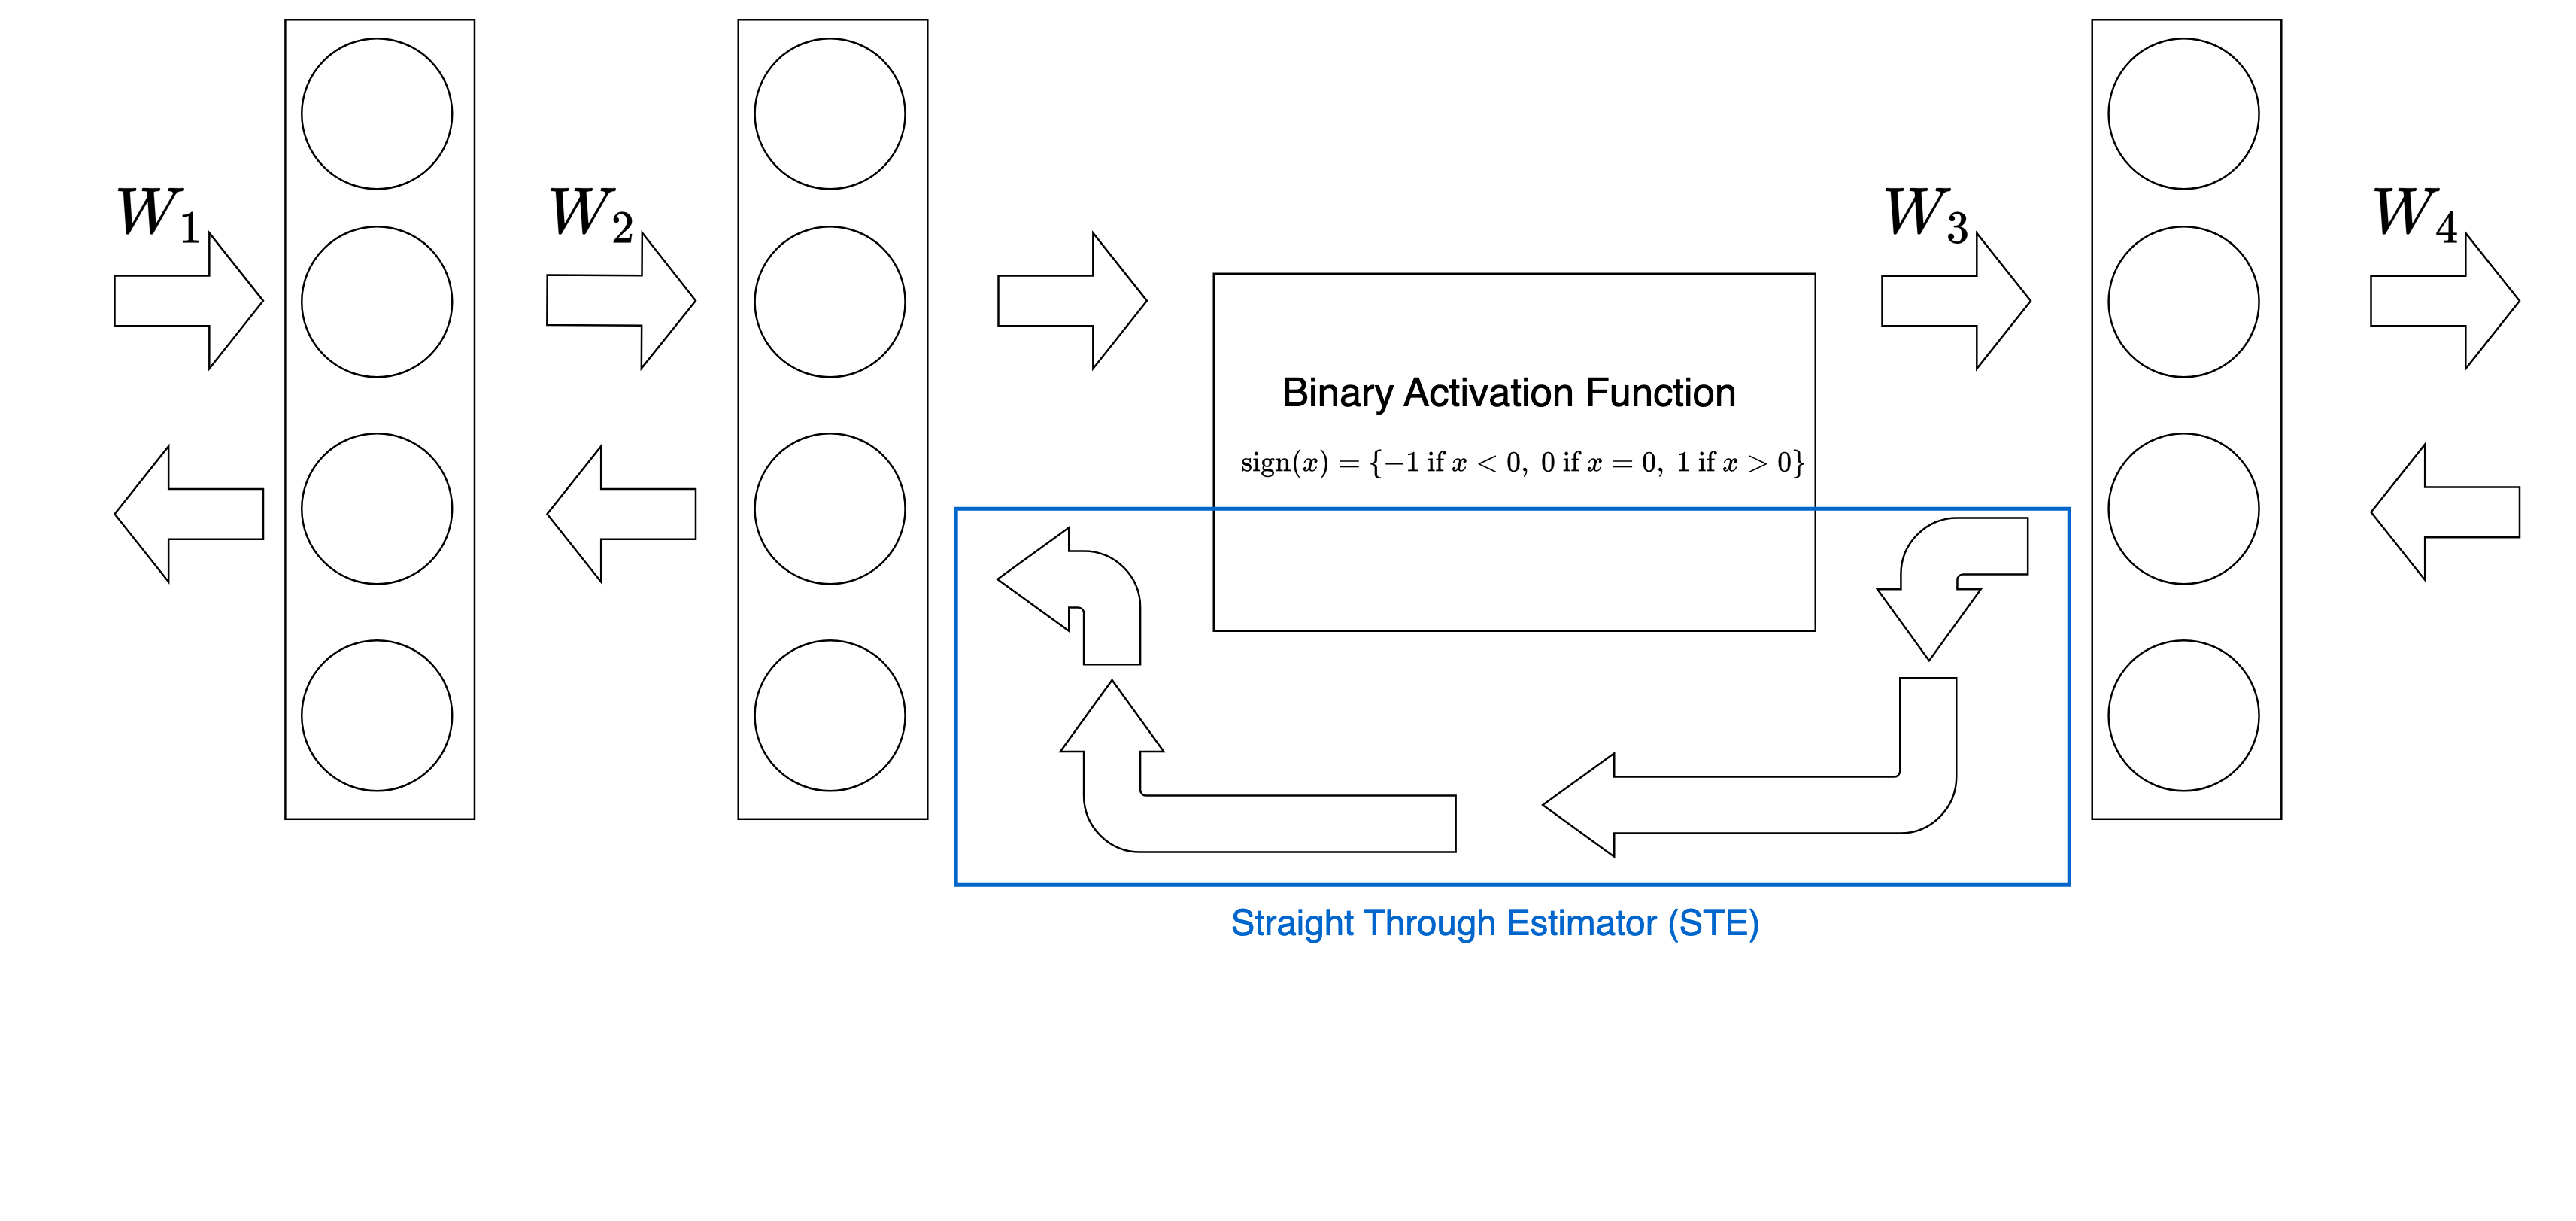
\includegraphics[width=0.9\textwidth]{figures/ste_diagram.jpg}
    \caption{Illustration of the Binary Activation Function and use of the Straight-Through Estimator (STE) in backpropagation.}
    \label{fig:ste_diagram}
\end{figure}

To solve this issue, BNNs use a method called the \textbf{Straight-Through Estimator (STE)}. Instead of using the true derivative of the sign function, STE pretends that the sign function behaves like the identity function during the backward pass. In other words, it bypasses the non-differentiable binarization step by assigning an approximate gradient.

The STE approximation is typically written as:
\[\frac{d}{dx} \text{sign}(x) \approx 
\begin{cases}
1, & |x| \leq 1 \\
0, & \text{otherwise}
\end{cases}\]
This means that if the input is within a certain range, the gradient is approximated as 1 and outside that range it is zero. This keeps gradients flowing during training and allows standard optimizers like Adam or AdaMax to work effectively.

This approach allows the network to continue updating its parameters, even though the actual gradient of the binarization step is not used. While the magnitude of the gradient may not be precise, STE preserves the direction of the update, which is often sufficient for convergence. As a result, BNNs can be trained using standard optimization algorithms, despite operating entirely on binary weights and activations during the forward pass.


\clearpage
\subsection{Batch Normalization and Activation Functions}
In Binary Neural Networks, the \textit{sign function} is used to binarize both weights and activations. However, this function is highly sensitive to its input values, particularly around zero. Small changes in the input can flip the sign and alter the binary output entirely. This makes it crucial to carefully control the distribution of inputs before binarization to ensure stable and meaningful outputs across layers.

To address this, \textit{Batch Normalization (BatchNorm)} is applied immediately before each binarization step. BatchNorm normalizes the input activations to have zero mean and unit variance across a mini-batch. This centers the data and keeps the values within a predictable range, making the binarization process more stable and reliable during training.

The batch normalization operation is defined as:
\[\text{BN}(x) = \gamma \cdot \frac{x - \mu_B}{\sqrt{\sigma_B^2 + \epsilon}} + \beta\]
Here, \( \mu_B \) and \( \sigma_B^2 \) represent the mean and variance of the input \(x\) over the batch. The terms \( \gamma \) and \( \beta \) are learnable parameters that allow the model to rescale and shift the normalized output. The small constant \( \epsilon \) is added to prevent division by zero. In BNN implementations that target hardware efficiency, the normalization is typically simplified by fixing \( \gamma = 1 \), \( \beta = 0 \) and disabling scaling during inference.

Once the input is normalized, it is binarized using the same sign function as before:
\[\text{sign}(\text{BN}(x)) = 
\begin{cases}
+1, & \text{BN}(x) \geq 0 \\
-1, & \text{BN}(x) < 0
\end{cases}\]
In BNNs, the combination of batch normalization and binarization replaces conventional activation functions such as ReLU. Rather than applying a separate non-linear function, the network uses the sign of the normalized activation to produce the binary output passed to the next layer.

By centering activations, BatchNorm prevents neurons from consistently outputting only +1 or −1, maintaining a balanced distribution of binary outputs. This promotes stable gradient flow during training, leading to faster convergence and improved model performance.


\clearpage
\subsection{Advantages and Trade-Offs}
Binary Neural Networks are designed to reduce computational cost, memory usage and power consumption by replacing floating-point operations with binary logic. These properties make BNNs especially suitable for deployment on resource-constrained hardware such as FPGAs.

\noindent\textbf{Memory Efficiency:} Since all weights and activations are stored using a single bit (\(-1\) or \(+1\)), the overall model size is reduced by a factor of 32 compared to networks that use 32-bit parameters. This allows for much smaller memory usage, which is particularly useful in embedded systems and edge devices.

\noindent\textbf{Computation Speed:} BNNs replace multiplication heavy operations with bitwise XNOR and popcount. These operations are faster and simpler to implement in hardware. As a result, inference latency is significantly reduced, especially when compared to conventional floating point neural networks.

\noindent\textbf{Power Efficiency:} Binary operations require less switching activity and fewer memory accesses, both of which reduce power usage. This makes BNNs well-suited for applications where energy efficiency is important, such as battery powered systems or real time low-power devices.

\noindent However, these advantages come with certain trade-offs:
\begin{itemize}
    \item \textbf{Accuracy Loss:} Binarization introduces approximation error by replacing real valued operations with binary ones. This can lower accuracy, particularly on complex or high resolution datasets.
    \item \textbf{Reduced Representational Power:} Binary weights and activations limit the expressiveness of each neuron. BNNs may require wider or deeper architectures to compensate for this reduction in capacity.
    \item \textbf{Difficult Hyperparameter Tuning:} Due to the aggressive quantization, BNNs are more sensitive to learning rates, batch sizes and initialization strategies, requiring more careful tuning during training.
    \item \textbf{Compatibility Issues:} Some standard deep learning layers and functions are not easily adapted to the binary domain, which can limit design flexibility or require custom implementations.
\end{itemize}



\clearpage
\section{Field Programmable Gate Arrays (FPGAs)}
Field Programmable Gate Arrays (FPGAs) are reconfigurable integrated circuits designed to implement custom digital logic. Unlike fixed function hardware like Application Specific Integrated Circuits (ASICs) or general purpose processors like CPUs and GPUs, FPGAs allow developers to define how the underlying hardware behaves even after the device has been manufactured. This flexibility enables precise control over timing, parallelism and data flow, which makes FPGAs suitable for applications requiring low latency, high throughput or hardware-level customization.

\subsection{Comparison with CPUs, GPUs and ASICs}
Traditional CPUs execute software instructions sequentially and are optimized for general purpose tasks. GPUs, while also programmable, are better suited for massively parallel workloads. ASICs on the other hand, are designed for a single, fixed function and provide optimal performance and power efficiency for that function, but they lack reconfigurability and require long development cycles.

FPGAs sit between general purpose processors and fixed-function hardware like ASICs. They offer better performance and power efficiency than CPUs and GPUs, while still being reconfigurable after manufacturing. This makes them a good choice for tasks like prototyping, signal processing, neural network inference and custom acceleration. However, using them effectively requires writing hardware-level code and designing the architecture carefully.

\clearpage
\subsection{Internal Structure of an FPGA}
An FPGA is composed of a regular array of logic and routing elements that can be programmed to implement a wide range of digital circuits. Its architecture is modular and consists of several key building blocks, as shown in Figure~\ref{fig:fpga_architecture}.

\begin{figure}[htbp]
    \centering
    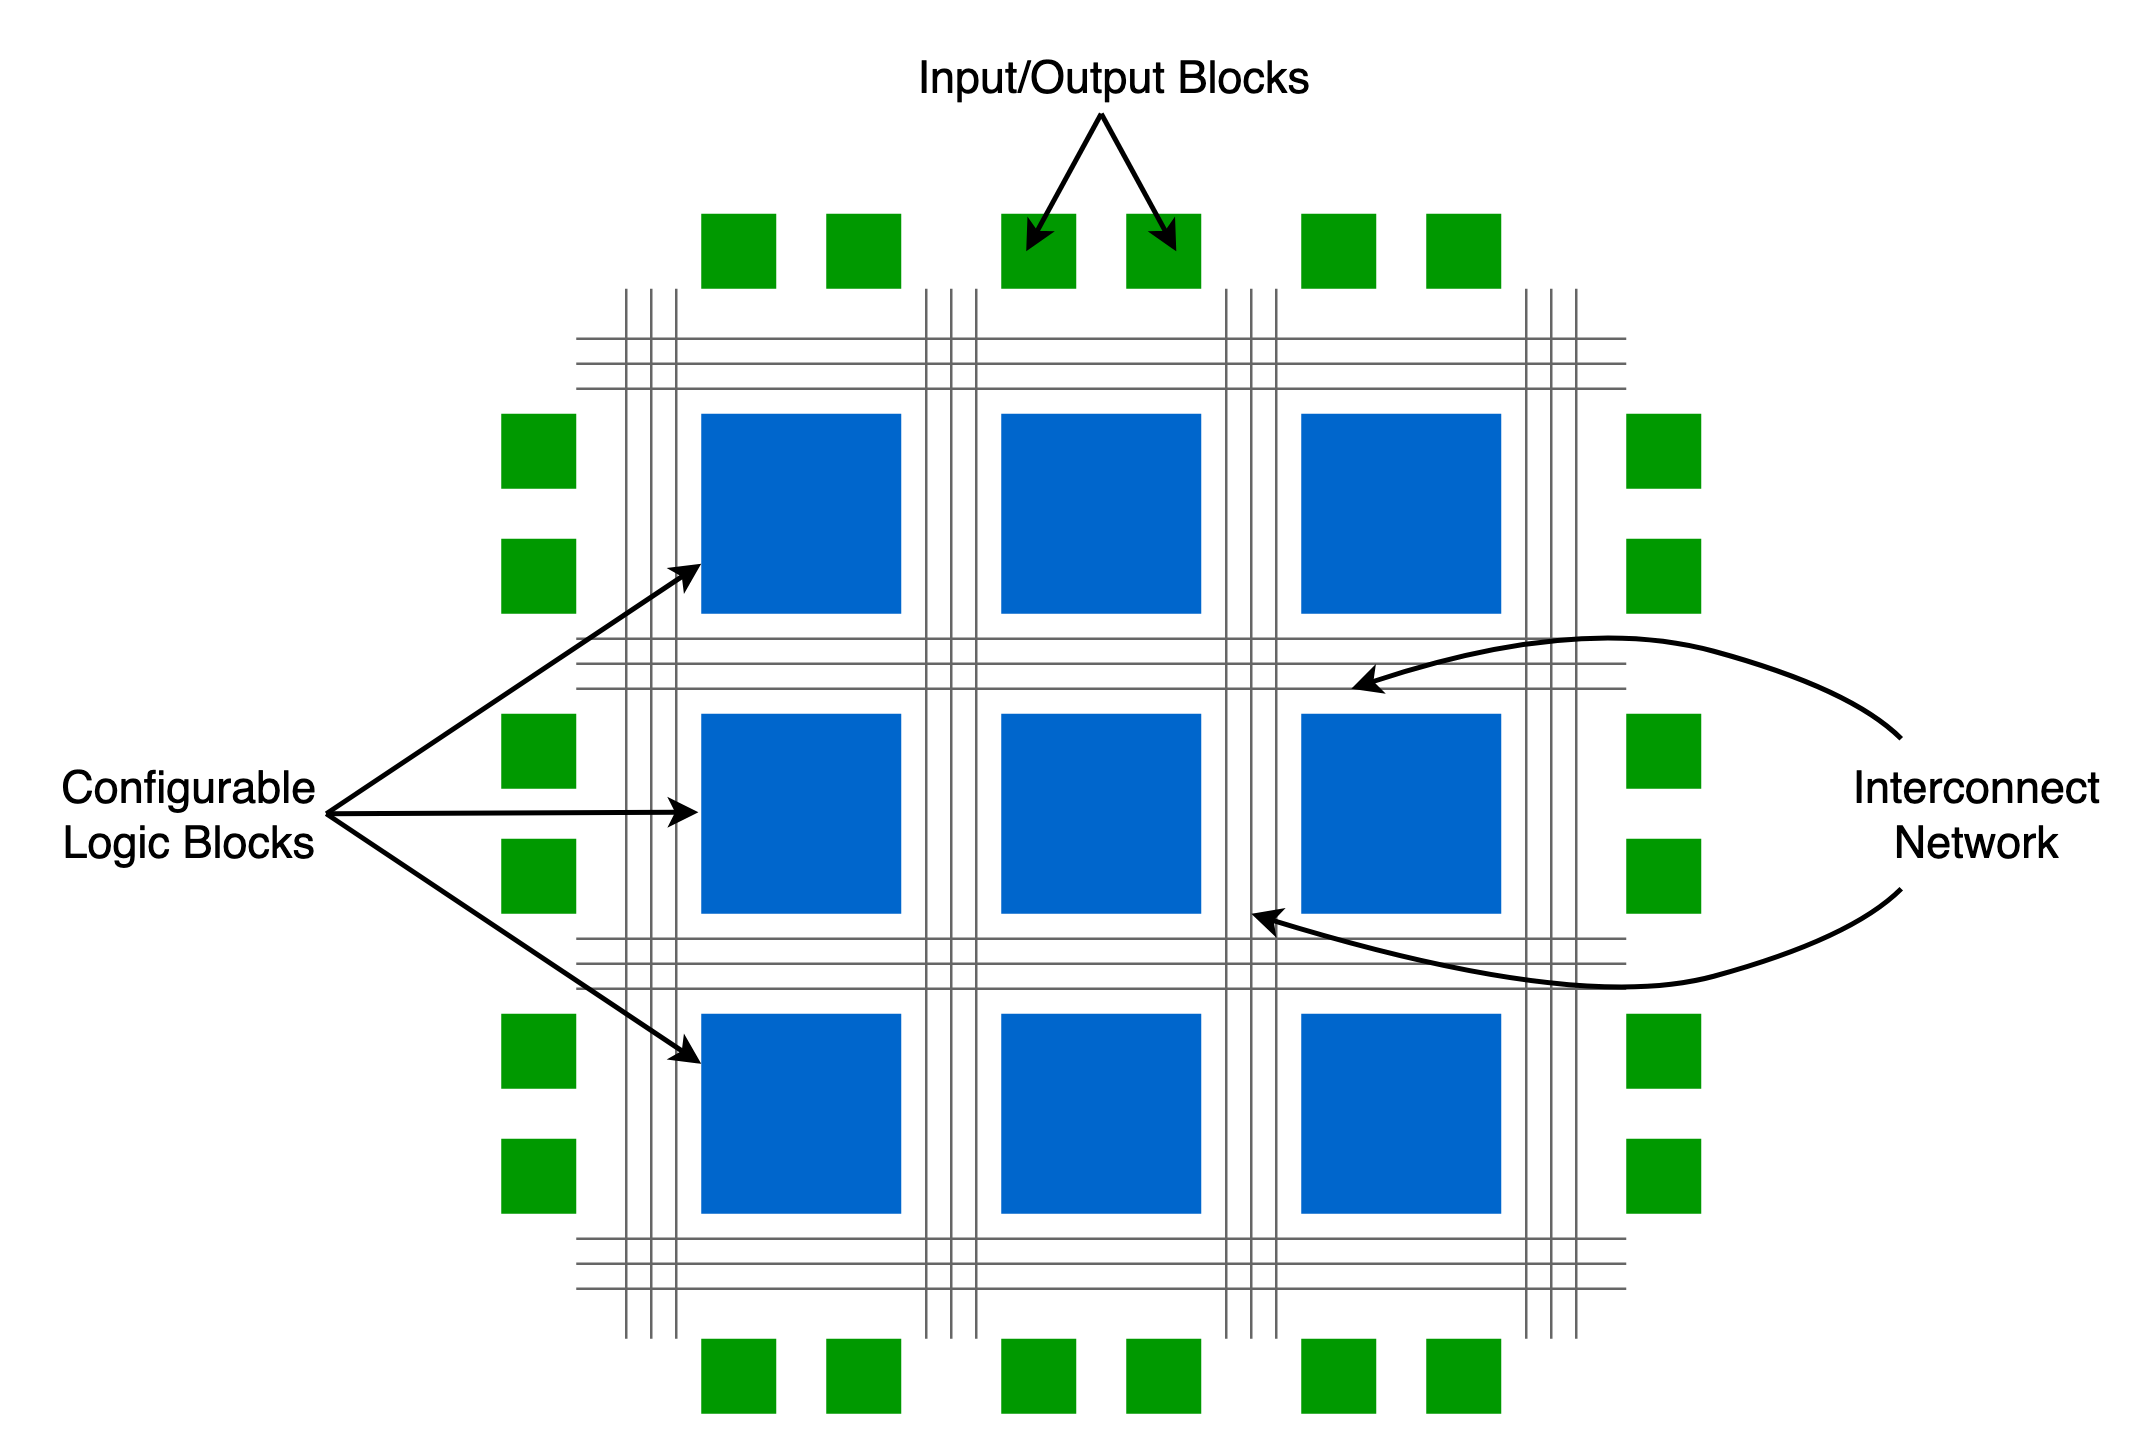
\includegraphics[width=0.8\textwidth]{figures/fpga_architecture.jpg}
    \caption{High-level layout of an FPGA showing Configurable Logic Blocks (CLBs), Input/Output Blocks (IOBs) and the interconnect network.}
    \label{fig:fpga_architecture}
\end{figure}

The main structural components of an FPGA include:

\textbf{1. Configurable Logic Blocks (CLBs):} \\ 
These are the main building blocks responsible for implementing logic functions. Each CLB contains multiple Look-Up Tables (LUTs) and flip-flops (FFs), which together enable both combinational and sequential logic. 
\begin{itemize}
    \item \textit{Look-Up Tables (LUTs):} Small memory arrays that store precomputed outputs for logic functions. A \(k\)-input LUT can implement any Boolean function of \(k\) variables. LUTs are what lead to the reconfigurability of FPGAs \cite[see p.~33]{1130285376382978560}.
    \item \textit{Flip-Flops (FFs):} 1-bit registers used to implement state-holding elements for sequential logic.
\end{itemize}
\begin{figure}[htbp]
    \centering
    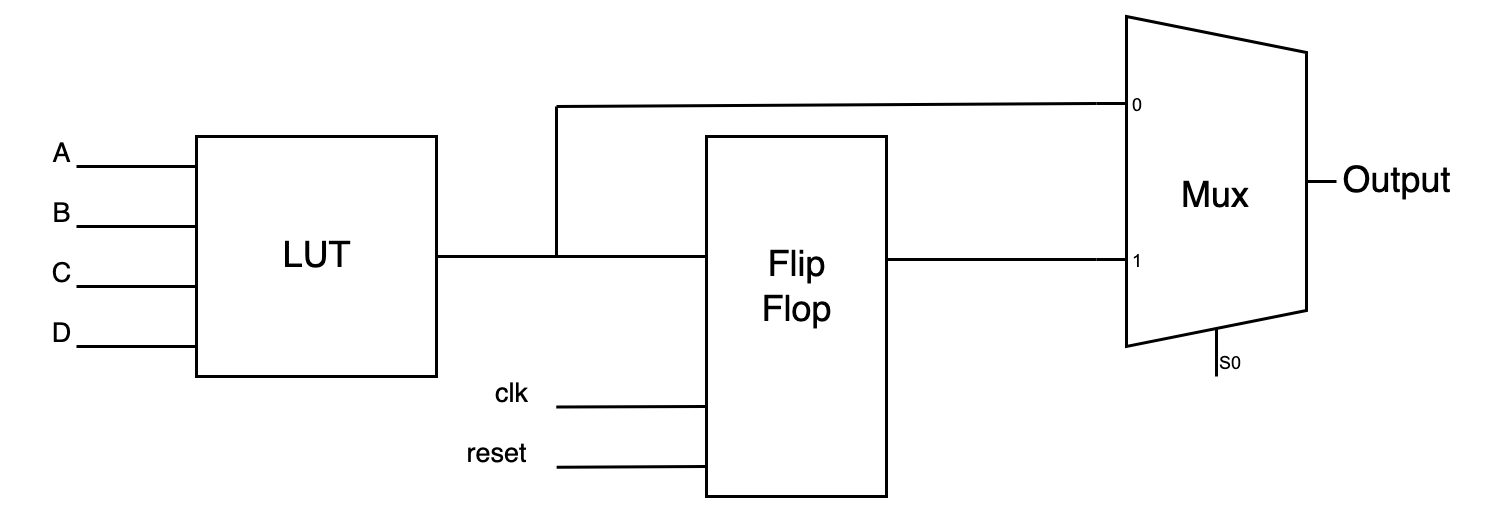
\includegraphics[width=0.6\textwidth]{figures/clb_diagram}
    \caption{Illustration of a Configurable Logic Block (CLB) containing LUTs and flip-flops.}
    \label{fig:clb_diagram}
\end{figure}
\FloatBarrier

\textbf{2. Interconnect Network:} \\
The interconnect fabric is a hierarchical and programmable wiring structure that allows logic blocks to be connected to each other or to I/O pins. It includes configurable switches, multiplexers and routing tracks. The flexibility of the interconnect enables the same physical fabric to implement very different designs. 

\textbf{3. Input/Output Blocks (IOBs):} \\ 
IOBs interface the FPGA with external signals. They support various I/O standards and can be configured as inputs, outputs or bidirectional ports.

\textbf{4. Dedicated Hardware Resources:} \\
Modern FPGAs include specialized blocks beyond the generic logic in CLBs. These blocks are optimized for common digital design tasks.
\begin{itemize}
    \item \textit{Block RAM (BRAM):} On-chip memory blocks that can be configured as single or dual-port RAMs. These are used to store buffers, image data or network weights, which is particularly useful in applications like BNNs where fast memory access is needed.
    \item \textit{DSP Slices:} Fixed function blocks designed for fast arithmetic operations such as multiplication, addition, accumulation and bit-shifting. These slices offload high speed math operations from CLBs, enabling efficient implementation of signal processing.
    \item \textit{Clocking Resources:} FPGAs include a network of global and regional clocks that distribute timing signals to different parts of the device. These networks ensure that all sequential elements operate in sync, even across large designs.
    \item \textit{Transceivers:} High speed serial interfaces for communication over protocols like PCIe or Ethernet. These allow FPGAs to interface directly with external high bandwidth devices or memory.
\end{itemize}

\subsection{Reconfigurability and Design Flow}
The term "field programmable" refers to the FPGA's ability to be configured after manufacturing. This is achieved by loading a bitstream file, generated by synthesis and implementation tools, into the FPGA. The design process typically includes:
\begin{itemize}
    \item Writing HDL code (such as Verilog or VHDL) to describe hardware behavior
    \item Synthesizing the HDL into logic primitives
    \item Mapping the logic to available resources (LUTs, FFs, BRAM, etc.)
    \item Placing and routing the design to satisfy timing constraints
    \item Generating and loading the bitstream onto the FPGA
\end{itemize}
This flow is slower and more complex than software compilation but results in highly optimized, parallel hardware tailored to the task.

\subsection{Advantages of FPGAs}
\begin{itemize}
    \item \textbf{Custom Parallelism:} Developers can design deeply pipelined or massively parallel data paths specific to their application.
    \item \textbf{Deterministic Latency:} Unlike CPUs and GPUs, FPGAs provide cycle accurate and predictable execution timing.
    \item \textbf{Reusability:} Designs can be updated, corrected or optimized after deployment without creating new hardware.
    \item \textbf{Power Efficiency:} For specific workloads, FPGAs can be more power efficient than CPUs or GPUs.
\end{itemize}

\subsection{Challenges and Limitations}
\begin{itemize}
    \item \textbf{Development Complexity:} FPGA design requires familiarity with hardware concepts and HDLs. Debugging and verifying designs is complex and more time consuming.
    \item \textbf{Lower Clock Speeds:} Compared to CPUs and ASICs, FPGAs generally operate at lower frequencies, which can limit throughput for sequential tasks.
    \item \textbf{Resource Constraints:} The number of LUTs, FFs, BRAMs and DSPs is limited, and must be carefully managed during design.
    \item \textbf{Compilation Overhead:} Synthesis and implementation steps are time consuming, often taking minutes to hours depending on design size.
\end{itemize}


\section{FPGA Deployment for Neural Networks}
As shown in \cite{Serrano:1100537}, FPGAs have historically been used in areas such as digital signal processing (DSP), control systems and data acquisition. In recent years, their role has expanded into machine learning applications due to their ability to implement custom dataflows and support low precision arithmetic. This is especially relevant for efficient neural network models such as Binary Neural Networks (BNNs), which rely on bitwise operations instead of floating point arithmetic.

At the same time, the growing interest in deep learning has led to increasingly complex models, often based on Convolutional Neural Networks (CNNs). These models typically use 32-bit floating point representations and consist of multiple layers, each with hundreds or thousands of neurons. While this depth improves predictive accuracy, it also significantly increases computational and memory demands, making it difficult to deploy these models on resource limited platforms.

Moreover, studies have shown that many deep networks contain significant parameter redundancy \cite{cheng2015explorationparameterredundancydeep}, suggesting that similar accuracy can be achieved with reduced precision or smaller models. This makes FPGAs a promising platform for deep learning acceleration, particularly in embedded and edge computing scenarios where efficiency and configurability are critical.

This redundancy presents a major barrier to hardware deployment, particularly on resource constrained platforms like FPGAs. However, BNNs provide a promising alternative to this challenge. These models can be designed in either fully connected or convolutional configurations and are particularly well suited for efficient FPGA implementation.

A practical and streamlined approach involves completing the training phase on conventional hardware (such as CPUs or GPUs), as training directly on FPGAs is both inefficient and difficult. Once the model is trained, the relevant parameters (binarized weights, activations and thresholds) can be extracted and loaded into the FPGA’s memory blocks. Inference operations, where inputs are processed using the trained parameters, can be executed on the FPGA in a highly parallel and resource efficient manner. In applications such as image classification or object recognition, the input image is first converted to a format compatible with the trained model, then passed to the FPGA, which computes the output using the optimized binary inference logic.


\section{Terms}
\begin{itemize}
    \item \textit{Binary Neural Network (BNN)} is a type of neural network in which both weights and activations are binarized, typically to values of +1 and -1. This allows for efficient computation using bitwise operations, reducing both memory usage and computational cost.

    \item \textit{Quantization-Aware Training (QAT)} is a training technique that accounts for quantization effects during both the forward and backward passes. It helps neural networks retain performance after being quantized for deployment in hardware environments.

    \item \textit{XNOR-Popcount} is the bitwise alternative to multiplication and addition in BNNs. The XNOR operation compares input and weight bits and popcount counts the number of ones, representing the similarity between inputs and weights.

    \item \textit{Threshold} in this project refers to a precomputed integer derived from batch normalization parameters. During inference, a neuron's output is compared against this threshold to decide whether it activates (1) or not (0).

    \item \textit{Finite State Machine (FSM)} is a control structure used in the Verilog implementation to coordinate each stage of inference. It defines states such as image loading, layer computation, output extraction and completion.

    \item \textit{ROM (Read-Only Memory)} is used to store binarized weights, thresholds and input images on the FPGA. These are loaded using \texttt{.mem} initialization files during simulation and deployment.

    \item \textit{Inference} refers to the process of making predictions with the trained model. In this project, inference is implemented entirely on the FPGA using custom Verilog logic to process input images and produce digit outputs.

    \item \textit{Simulation} is the process of verifying the design before hardware deployment. Functional simulations with waveform analysis were used to debug signal behavior, control flow and output correctness.
\end{itemize}
\clearpage

\section{Motivation}

\subsection{Accessibility}
Because it doesn’t need powerful hardware, a BNN on an FPGA is a very accessible solution. It can be used in many areas where power or space is limited. Since the hardware design stays the same, the only thing needed to change its purpose is to train it with a new dataset. This makes the system flexible and easy to repurpose for other tasks.

\subsection{Transparency and Control}
Most similar projects use high-level tools like HLS or built-in IP blocks, which hide how things actually work behind the scenes. In this project, everything is written in Verilog from scratch. The logic, timing and data flow are all designed manually. This gives full control and a clearer understanding of how neural networks can be implemented directly in hardware.

\subsection{Real-Time Inference}
One of the key strengths of implementing a BNN on an FPGA is the ability to perform inference in real time. Unlike traditional CPUs or GPUs, where inference can be delayed due to operating system overhead and batch processing, an FPGA can deliver consistent, low latency results. This makes it highly suitable for scenarios like sensor data processing, interactive systems or embedded controllers where fast responses are critical.


\section{Efficiency and Hardware Optimization}

To achieve real time inference and minimize hardware usage, the Verilog implementation of the BNN was carefully optimized at the structural level. Unlike software based approaches that rely on abstract layers and general purpose logic, this design uses bit level operations mapped directly to hardware components.

The core operations, such as XNOR and popcount, are performed using bitwise and arithmetic logic inside a sequential Finite State Machine (FSM) based control structure. This avoids unnecessary arithmetic overhead. By restricting all activations and weights to 1 bit values, the design eliminates multipliers entirely, which are expensive in terms of logic and power. Instead, logic gates and simple counters are used to compute dot products and compare them against learned thresholds.

Layer wise inference is coordinated through a single FSM, where each state corresponds to a specific stage in the pipeline. This structure enables predictable control flow with minimal latency and clearly defined signal transitions.

The entire computation path is constructed using static ROM-based memory modules to preload weights, thresholds and test images. This makes the design highly predictable and free from control overhead typically found in processor based systems.

From synthesis to implementation, hardware constraints such as LUT usage and clock timing were considered to ensure that the design fits comfortably within the available FPGA resources. The final implementation uses minimal logic slices, no DSP blocks and only a small fraction of available BRAM, showing that efficient BNN inference is achievable on mid range FPGA platforms without resorting to high-level synthesis.


\section{Scope and Limitations}
This project focuses exclusively on the inference stage of a pre-trained BNN, implemented from scratch in Verilog for deployment on the Nexys A7-100T FPGA board. It covers the full process from model export and weight binarization to simulation, synthesis and real time prediction. The model is designed for classification of 28$\times$28 grayscale handwritten digits from the MNIST dataset and inference results are displayed directly on a seven-segment interface. All components are developed without high level synthesis (HLS), enabling precise control over the logic.

However, the implementation is limited in several respects. First, the BNN architecture used is fully connected and fixed in size, meaning it cannot currently support convolutional layers or dynamic reconfiguration without modifying the hardware. Second, only a fixed number of input images can be tested at a time, since images are stored statically in ROM. Third, the system is optimized for correctness and simplicity rather than maximum speed or resource utilization. Although the FSM based control ensures deterministic behavior and simple parallelism, it does not yet include pipelining or advanced parallelism. Finally, training is performed offline using Python and TensorFlow and this workflow assumes access to floating-point compute resources during the training phase.


\section{Problem Definition}
While BNNs have great potential for efficient inference, most existing hardware implementations rely on high-level tools. These approaches limit visibility into how data flows through the network and how decisions are made at the hardware level. Many also skip Quantization-Aware Training (QAT), which can result in reduced accuracy after deployment.

This project aims to implement a trained BNN for handwritten digit recognition entirely in Verilog, with no abstraction layers. The goal is to design and verify a bit-accurate inference system that runs on an FPGA with full control over each stage of computation. The challenge lies in building a custom pipeline from scratch, including weight loading, XNOR-popcount logic, thresholding and FSM-based control, all while preserving the efficiency benefits of a binarized model. The final system should deliver correct predictions in real time, using compact hardware and minimal memory.

\section{Requirements}

The implementation of a BNN on FPGA requires both software-side and hardware-side considerations:
\begin{itemize}
    \item \textit{Trained BNN Model:} A fully trained BNN with binarized weights and activations. The model must be compatible with quantization-aware deployment and produce predictable, stable inference results.
    
    \item \textit{Threshold Extraction:} Batch normalization parameters must be available and convertible into discrete thresholds that can be used during FPGA inference.

    \item \textit{Weight and Threshold Encoding:} All model weights and thresholds must be exported into binary \texttt{.mem} files for integration with ROM modules on the FPGA.

    \item \textit{FPGA Platform:} A target FPGA board capable of storing the model and performing real time inference. In this project, the Nexys A7-100T board is used, which includes sufficient LUTs, flip-flops and BRAM.

    \item \textit{Memory and Logic Resources:} Sufficent on-chip resources to store intermediate outputs (activation buffers) and support popcount logic, XNOR operations and FSM control.

    \item \textit{Toolchain Support:} Xilinx Vivado must support simulation, synthesis and programming for the selected FPGA, and allow loading of external memory contents through \texttt{.mem} files.

    \item \textit{Test Inputs:} Input images must be converted to binarized format and structured into ROM for simulation and on-board testing.

    \item \textit{Output Interface:} A functional seven-segment display interface is required to show the predicted digit during real-time inference.

    \item \textit{Verification Environment:} A working testbench with support for image testing and waveform inspection is needed for design validation and debugging.
\end{itemize}


% CHAPTER 2 - BACKGROUND
% -------------------------
\clearpage
\chapter{BACKGROUND}
\label{background}

\section{Previous Works}
Binary Neural Networks (BNNs) offer an efficient alternative to traditional deep learning models in resource constrained hardware environments. Courbariaux, Hubara, Soudry, El-Yaniv, and Bengio \cite{courbariaux2016binarizedneuralnetworkstraining} introduced a training method where both weights and activations are binarized. This replaced standard floating-point operations with bitwise XNORs and popcounts, reducing memory usage and computational overhead by an order of magnitude. Their work became a foundation for many hardware oriented neural network designs.

Several frameworks, including Xilinx FINN \cite{10.1145/3020078.3021744}, have explored FPGA-based deployment of BNNs. These efforts typically use high-level synthesis and stream-based dataflows. While they demonstrate low-latency and energy efficient inference, they often abstract away internal logic, making precise control over computation more difficult.

MNIST is a common benchmark for digit recognition. Most solutions rely on quantized or full-precision convolutional networks. However, BNN-based models remain appealing due to their minimal use of resources. Their inference pipelines consist only of binary arithmetic, making them well-suited for hardware execution.

Unlike many designs that avoid Quantization-Aware Training (QAT) or depend on automated tools, this project implements a QAT-trained BNN in Verilog, featuring manual control of bit-level data, finite state machines, and thresholding logic for a clear hardware pipeline.



% CHAPTER 3 - Analysis & Design
% -------------------------
\clearpage
\chapter{ANALYSIS \& DESIGN}
\label{chapter:analysis_and_design}

% Analysis part
% -------------------------
\section{Functional Requirements}
\begin{enumerate}[label=(\roman*)]
    \item \textbf{Input Acquisition and Binarization}
    \begin{itemize}
        \item The system must accept 28$\times$28 grayscale images converted offline into 1-bit binary form, compatible with the pre-trained model’s input format, and load them into ROMs for inference.
    \end{itemize}
    
    \item \textbf{XNOR-Popcount Based Layer Computation}
    \begin{itemize}
        \item The system must compute binary matrix multiplications using XNOR and popcount operations.
        \item Each layer must perform threshold comparisons using precomputed thresholds.
    \end{itemize}
    
    \item \textbf{Parallel Inference Execution}
    \begin{itemize}
        \item The system must support variable levels of neuron parallelism.
        \item Finite State Machine logic must coordinate the sequential processing of neuron batches within each layer.
    \end{itemize}
    
    \item \textbf{Weight and Threshold Memory Access}
    \begin{itemize}
        \item The system must access weights using dual-port ROMs instantiated from .mem files and optimized for parallel reads.
        \item Thresholds must be retrieved from single-port ROMs stored as signed integer values.
    \end{itemize}
    
    \item \textbf{Digit Prediction Output}
    \begin{itemize}
        \item The system must compute a 4-bit digit output via an argmax logic over final layer scores.
    \end{itemize}
    
    \item \textbf{Correctness}
    \begin{itemize}
        \item The inference result must match expected predictions from the trained model.
    \end{itemize}
    
    \item \textbf{Real-Time Response}
    \begin{itemize}
        \item The system must complete inference within a bounded latency ($<0.02$ ms at 80 MHz for up to 64-level parallelism).
    \end{itemize}
\end{enumerate}

\clearpage
\section{Nonfunctional Requirements}
\begin{enumerate}[label=(\roman*)]
    \item \textbf{Performance}
    \begin{itemize}
        \item The system must operate with minimal latency across tested parallelization levels.
        \item Throughput must be sufficient for real-time classification on the Nexys A7 FPGA at 80 MHz.
    \end{itemize}

    \item \textbf{Scalability}
    \begin{itemize}
        \item The design must support different levels of parallelism via parametrization without structural rewrites.
    \end{itemize}

    \item \textbf{Resource Efficiency}
    \begin{itemize}
        \item The system must utilize only the minimum number of memory and logic blocks necessary to support a given parallelization level, ensuring no redundant ROM instantiations or unused modules.
    \end{itemize}

    \item \textbf{Portability}
    \begin{itemize}
        \item The project must be deployable on other mid-tier FPGA boards with minimal changes, assuming similar resource profiles.
    \end{itemize}
    
    \item \textbf{Maintainability and Extensibility}
    \begin{itemize}
        \item The Verilog implementation must remain modular, with clearly separated modules for FSM, memory, computation and display logic.
    \end{itemize}

    \item \textbf{Verification and Simulation}
    \begin{itemize}
        \item A testbench must be maintained for simulation based waveform inspection and debugging.
        \item Simulation results must confirm that the hardware inference outputs match the predictions of the trained model, achieving accuracy consistent with the model's baseline performance.
    \end{itemize}

    \item \textbf{Usability}
    \begin{itemize}
        \item The design must include visual output via seven-segment display to confirm inference predictions on hardware.
    \end{itemize}

    \item \textbf{Compliance}
    \begin{itemize}
        \item The design must conform to synchronous digital design practices using standard Verilog and Xilinx Vivado toolchain.
    \end{itemize}
\end{enumerate}

\clearpage
\section{BNN vs CNN Comparison}
Two neural network models were trained and evaluated for the task of handwritten digit classification. Both were implemented in TensorFlow with fixed random seeds and tested under identical conditions. One uses a binarized fully connected architecture (BNN), while the other follows a standard convolutional structure (CNN). While both models perform the same task and operate on the same input format, they differ significantly in architecture, computational cost and hardware suitability.

\subsection{Accuracy}
The CNN achieved a final test accuracy of \textbf{99.31\%}, whereas the BNN reached \textbf{87.97\%}. This result highlights the strength of convolutional layers in extracting spatial features from images. By using localized filters and hierarchical representation learning, the CNN is able to generalize better and make better predictions. In contrast, the BNN flattens all spatial structure at the input and applies binary linear transformations, which limits its ability to distinguish between visually similar digits. The 11.34\% difference in accuracy reflects this architectural limitation and suggests that the BNN sacrifices accuracy for simplicity.

\subsection{Inference Time}
Mean inference latency over 100 CPU runs was \textbf{15.71 ms} for the BNN and \textbf{16.36 ms} for the CNN. Although the average runtime difference is small, the CNN showed significantly higher variance, with its maximum latency reaching 46.75 ms. The BNN remained tightly between 14.69 ms and 18.19 ms. This consistency is the result of its regular structure and deterministic computation path. The CNN, on the other hand, contains multiple non-linear operations, variable memory access patterns and control flow variations due to dropout and activation layers.

From a deployment perspective, this variability can pose a problem in real-time systems where predictable timing is required. Even though the CNN is slightly slower on average, the greater latency spread introduces uncertainty. In contrast, the BNN offers stable and bounded performance.
\begin{table}[htbp]
    \centering
    \begin{tabular}{|c|c|c|c|c|}
        \hline
        \textbf{Model} & \textbf{Mean (ms)} & \textbf{Min (ms)} & \textbf{Max (ms)} & \textbf{Std Dev (ms)} \\
        \hline
        BNN & 15.71 & 14.69 & 18.19 & 0.65 \\
        \hline
        CNN & 16.36 & 14.87 & 46.75 & 3.15 \\
        \hline
    \end{tabular}
    \vspace{0.5\baselineskip}
    \caption{CPU inference latency statistics across 100 runs.}
    \label{table:cpu_inference_latency}
\end{table}

\subsection{Model Size}
The saved BNN model occupies \textbf{1.4 MB} of storage, while the CNN model occupies \textbf{2.7 MB} of storage. This double increase in model size reflects the CNN’s use of full-precision weights and the higher number of parameters introduced by convolutional filters and dense layers. In contrast, the BNN represents each weight with a single bit and ignores bias terms entirely. As a result, the BNN is more compact and efficient to store and transfer.

\subsection{Training Time}
Training the BNN for 15 epochs took \textbf{15 seconds}, whereas the CNN required \textbf{71 seconds} for just 10 epochs. Even after adjusting for the difference in epoch count, the CNN remains considerably slower to train. This is expected because convolutional operations are more computationally expensive than simple binary matrix multiplications. Additionally, the CNN's use of dropout, activation functions and floating-point arithmetic increases training time. 

The speed of BNN training allows for more rapid iteration during development, particularly when tuning hyperparameters or re-training on new datasets. On the other hand, the CNN requires fewer epochs to converge due to its feature extraction capacity.

\subsection{Architectural Complexity}
The CNN consists of two convolutional layers with ReLU activation, two max pooling layers, a fully connected layer with dropout and a softmax output. This structure enables the model to extract and combine spatial features across multiple scales, but it also introduces significant complexity. Inference requires floating-point multiplications, activation evaluations and large intermediate feature maps.

The BNN consists of three fully connected layers without bias, each followed by batch normalization. All weights and activations are binary and inference relies on XNOR-popcount operations followed by threshold comparison. This regular and uniform structure makes the model much easier to map to hardware. Memory accesses are predictable, computation paths are short and no multipliers are required.

\subsection{Suitability for FPGA}
The BNN maps directly to FPGA resources. Its bitwise operations can be efficiently implemented using LUTs and the absence of multipliers allows the design to avoid using DSP blocks entirely. The lack of architectural branching and the consistent layer pattern simplify FSM design and make parallelization simple. This allows fine control over latency and resource usage during hardware implementation.

In contrast, the CNN’s convolution layers require multiply-accumulate logic and intermediate buffers, which must either be implemented using DSP slices or emulated using logic blocks, both of which increase complexity. Furthermore, the irregular control flow and dynamic range of floating-point arithmetic introduce challenges in timing closure and memory management.

While the CNN delivers better accuracy, its computational requirements make it less suitable for resource-constrained hardware. The BNN provides a better trade-off between accuracy, speed and implementation cost, especially for applications where deterministic latency and low power consumption are more important than top-tier accuracy.

\clearpage
\section{Platform Comparison: FPGA, ASIC, CPU, GPU}
Selecting an appropriate computational platform is essential for deploying embedded machine learning models such as BNNs, especially in environments where real-time inference, hardware cost and resource utilization are critical factors. This section provides a comparative evaluation of four key platforms; CPU, GPU, ASIC and FPGA, based on several dimensions including performance, flexibility, development complexity and cost. 

\subsection{CPU (Central Processing Unit)}
The CPU is a general-purpose processor capable of executing a wide range of instructions in a sequential or moderately parallel manner. It is the most accessible processing unit in terms of both cost and development tools and serves as the backbone of conventional computing systems.

CPUs offer easy implementation and rapid deployment but are not optimized for highly parallelized workloads like matrix-heavy BNN inference. While multi-core and multi-threaded architectures can handle modest parallelism, the overall speed for bitwise operations like XNOR-popcount is limited.
\begin{itemize}
    \item \textbf{Initial Cost:} Low. Commodity CPUs are widely available in the \$100-\$400 range.
    \item \textbf{Development Time:} Very short. High-level languages and software stacks allow immediate prototyping.
    \item \textbf{Parallelism:} Moderate. Typically supports 4-16 threads with shared memory, limiting scalability for high-throughput tasks.
    \item \textbf{Inference Latency:} Moderate. Suitable for prototyping or low-frequency tasks but not optimal for real-time systems.
    \item \textbf{Energy Efficiency:} Low for parallel tasks. Power consumption increases significantly with workload size.
    \item \textbf{Suitability for BNNs:} Acceptable for validation or CPU based benchmarking, but not viable for deployment at scale.
\end{itemize}

\subsection{GPU (Graphics Processing Unit)}
GPUs consist of thousands of smaller cores designed to handle parallel workloads efficiently. They were originally developed for graphics rendering but their architecture has been repurposed for general-purpose computationally intensive tasks, especially in deep learning.

GPUs offer high throughput for neural networks and excel in floating-point operations. However, BNNs operate primarily on bitwise logic, which is not natively optimized on GPU hardware. Additionally, the overhead of data transfer between host and device memory can become a bottleneck in latency sensitive applications.
\begin{itemize}
    \item \textbf{Initial Cost:} Moderate to high. High-end GPUs cost between \$1,000 and \$10,000.
    \item \textbf{Development Time:} Moderate. Frameworks like CUDA, PyTorch and TensorFlow accelerate development but require some learning curve.
    \item \textbf{Parallelism:} Very high. Thousands of threads can be executed concurrently, ideal for large scale training.
    \item \textbf{Inference Latency:} Low to moderate. Fast for batch processing but suboptimal for single-sample, low-latency inference.
    \item \textbf{Energy Efficiency:} Moderate. High compute density but power usage scales with workload and memory usage.
    \item \textbf{Suitability for BNNs:} Good for training or batch inference but not optimal for lightweight, real-time applications.
\end{itemize}

\subsection{ASIC (Application-Specific Integrated Circuit)}
ASICs are custom designed chips fabricated to perform a specific task with extreme efficiency. Inference on an ASIC is typically orders of magnitude faster than on general purpose hardware due to dedicated logic for every operation.

Despite their performance, ASICs suffer from lack of flexibility. Any change in model structure or logic requires a new fabrication cycle. Moreover, ASIC development involves high non-recurring engineering (NRE) costs and extended lead times.
\begin{itemize}
    \item \textbf{Initial Cost:} Extremely high. NRE costs can range from \$100,000 to several million dollars depending on complexity.
    \item \textbf{Per-Unit Cost (High Volume):} Very low. Once produced, ASICs can cost as little as \$5-\$20 per chip in mass production.
    \item \textbf{Development Time:} Long. Typical design and tape-out cycles exceed 6 months.
    \item \textbf{Parallelism:} Maximum. Entire BNN pipeline can be hardwired into the chip.
    \item \textbf{Inference Latency:} Ultra-low. ASICs provide deterministic, cycle-level latency.
    \item \textbf{Energy Efficiency:} Highest. Tailored dataflow and power gating yield unmatched performance-per-watt.
    \item \textbf{Suitability for BNNs:} Ideal for commercial deployment at massive scale, but impractical for research or evolving models.
\end{itemize}

\subsection{FPGA (Field-Programmable Gate Array)}
FPGAs offer a reconfigurable fabric of logic blocks that can be tailored for specific workloads post-manufacturing. This allows for customized data paths, pipelining and parallelism, making FPGAs particularly effective for BNNs, where the majority of operations are binary.
\begin{itemize}
    \item \textbf{Initial Cost:} Low to moderate. Boards like the Basys 3 and Nexys A7 are priced around \$150-\$400 with no NRE overhead.
    \item \textbf{Development Time:} Moderate. Verilog/VHDL design and synthesis flows require hardware familiarity.
    \item \textbf{Parallelism:} Configurable. Varies with resource availability.
    \item \textbf{Inference Latency:} Very low. Measured latencies reach real-time benchmarks.
    \item \textbf{Energy Efficiency:} High for bitwise workloads. Unused logic can be disabled during synthesis.
    \item \textbf{Suitability for BNNs:} Excellent. Especially valuable in research, edge deployment and model-specific customization.
\end{itemize}

\subsection{Conclusion}
Each platform offers unique advantages depending on the target use case. CPUs and GPUs provide accessibility and easy development but fall short in latency critical or resource-constrained environments. ASICs outperform all others in raw efficiency but are suitable only for mass production due to high non-recurring engineering costs and lack of reconfigurability.

FPGAs achieve a practical balance between flexibility, speed and resource utilization. They allow hardware level customizations such as adjusting the level of parallelism and optimizing bitwise operations, which are essential for efficient BNN inference. Furthermore, their reprogrammable nature makes them exceptionally well-suited for supporting a variety of trained neural network models, including those with different depths, layer configurations and neuron counts. This adaptability is especially valuable in development and research settings, where architectural changes and retraining are frequent. 

The experimental platform-specific results such as including inference time, resource utilization and power estimates are presented in Chapter~\ref{chapter:test_and_results}.


% Design part
% -------------------------
\clearpage
\section{Input Preprocessing and Dataset}
In this project, the MNIST dataset was used as the primary source of input data. It consists of 60,000 training images and 10,000 test images, each representing a handwritten digit between 0 and 9. Every image is a grayscale 28×28 pixel matrix, resulting in 784 pixel values per sample.

The dataset was chosen because of its simplicity and wide use in evaluating classification models, particularly for digit recognition tasks. Its low resolution and clearly defined labels make it ideal for training lightweight neural networks such as Binary Neural Networks (BNNs), which are optimized for resource-constrained hardware.

Before feeding the data into the model, all pixel values were normalized to the range of -1 to 1. This normalization is important for compatibility with the binarization functions used in BNNs. Additionally, the input images were reshaped into one-dimensional vectors to fit the dense layer based model architecture used in this work.

\section{Binary Neural Network Architecture}
The architecture of the BNN designed for this project is detailed in Table~\ref{table:bnn_architecture}. The network follows a simple but highly efficient structure using fully connected (\texttt{Dense}) layers combined with binarization at both the weight and activation levels.

The input to the network consists of 28$\times$28 grayscale images from the MNIST dataset which are flattened into 784 dimensional vectors. These vectors are inputs to the first fully connected layer, which maps the 784 input features to 128 binary activations. Both the weights and activations at this stage are binarized using the sign function and batch normalization is applied to the outputs to stabilize training.

The second layer takes the 128 dimensional binary activations and produces 64 binary activations through another fully connected binarized layer. Similar to the first layer, batch normalization is applied to maintain training stability.

The final layer maps the 64 binary features to 10 outputs, corresponding to the ten digit classes (0–9). Unlike the hidden layers, the output layer does not apply an activation function after the dense operation. Instead, the outputs are left as raw logits, which are later processed using a softmax activation during evaluation or classification.

All weight parameters in the hidden and output layers are binarized to 1-bit precision which significantly reduces the memory usage and computational complexity of the network. The activations are also binarized in the hidden layers.
\begin{table}[htbp]
    \centering
    \resizebox{\textwidth}{!}{%
    \begin{tabular}{|c|c|c|c|c|c|c|}
        \hline
        \textbf{Layer} & \textbf{Type} & \textbf{Input Size} & \textbf{Output Size} & \textbf{Weight Precision} & \textbf{Activation Function} \\
        \hline
        Input Layer & -- & 28$\times$28 grayscale & 784 (flattened) & -- & -- \\
        \hline
        Dense Layer 1 & Fully Connected & 784 & 128 & 1-bit & Sign + BatchNorm \\
        \hline
        Dense Layer 2 & Fully Connected & 128 & 64 & 1-bit & Sign + BatchNorm \\
        \hline
        Output Layer & Fully Connected & 64 & 10 & 1-bit & None (raw logits) \\
        \hline
    \end{tabular}%
    }
    \vspace{0.5\baselineskip}
    \caption{Detailed Architecture of the Binary Neural Network Used in This Project}
    \label{table:bnn_architecture}
\end{table}

\clearpage
\section{Inference Pipeline Design}
The inference pipeline starts from the input image and progresses through binary matrix operations at each layer. For every neuron, the activations from the previous layer are XNORed with the binarized weights. The XNOR results are passed through a popcount operation, which counts the number of matching bits.

The popcount value is then compared with a predefined threshold specific to each neuron. If the popcount exceeds the threshold, the neuron output is set to 1; otherwise, it is set to 0. This process replaces standard activation functions with a binary decision step based on thresholds.

Intermediate outputs between the layers are kept in binary form, keeping the compactness and reducing memory and computation requirements. In the final output layer, the results are stored as integer scores rather than binary outputs, allowing the predicted class to be determined with increased accuracy.

The inference pseudocode summarizing these steps is shown in Figure~\ref{fig:bnn_inference_pseudocode}.
\begin{figure}[htbp]
    \centering
    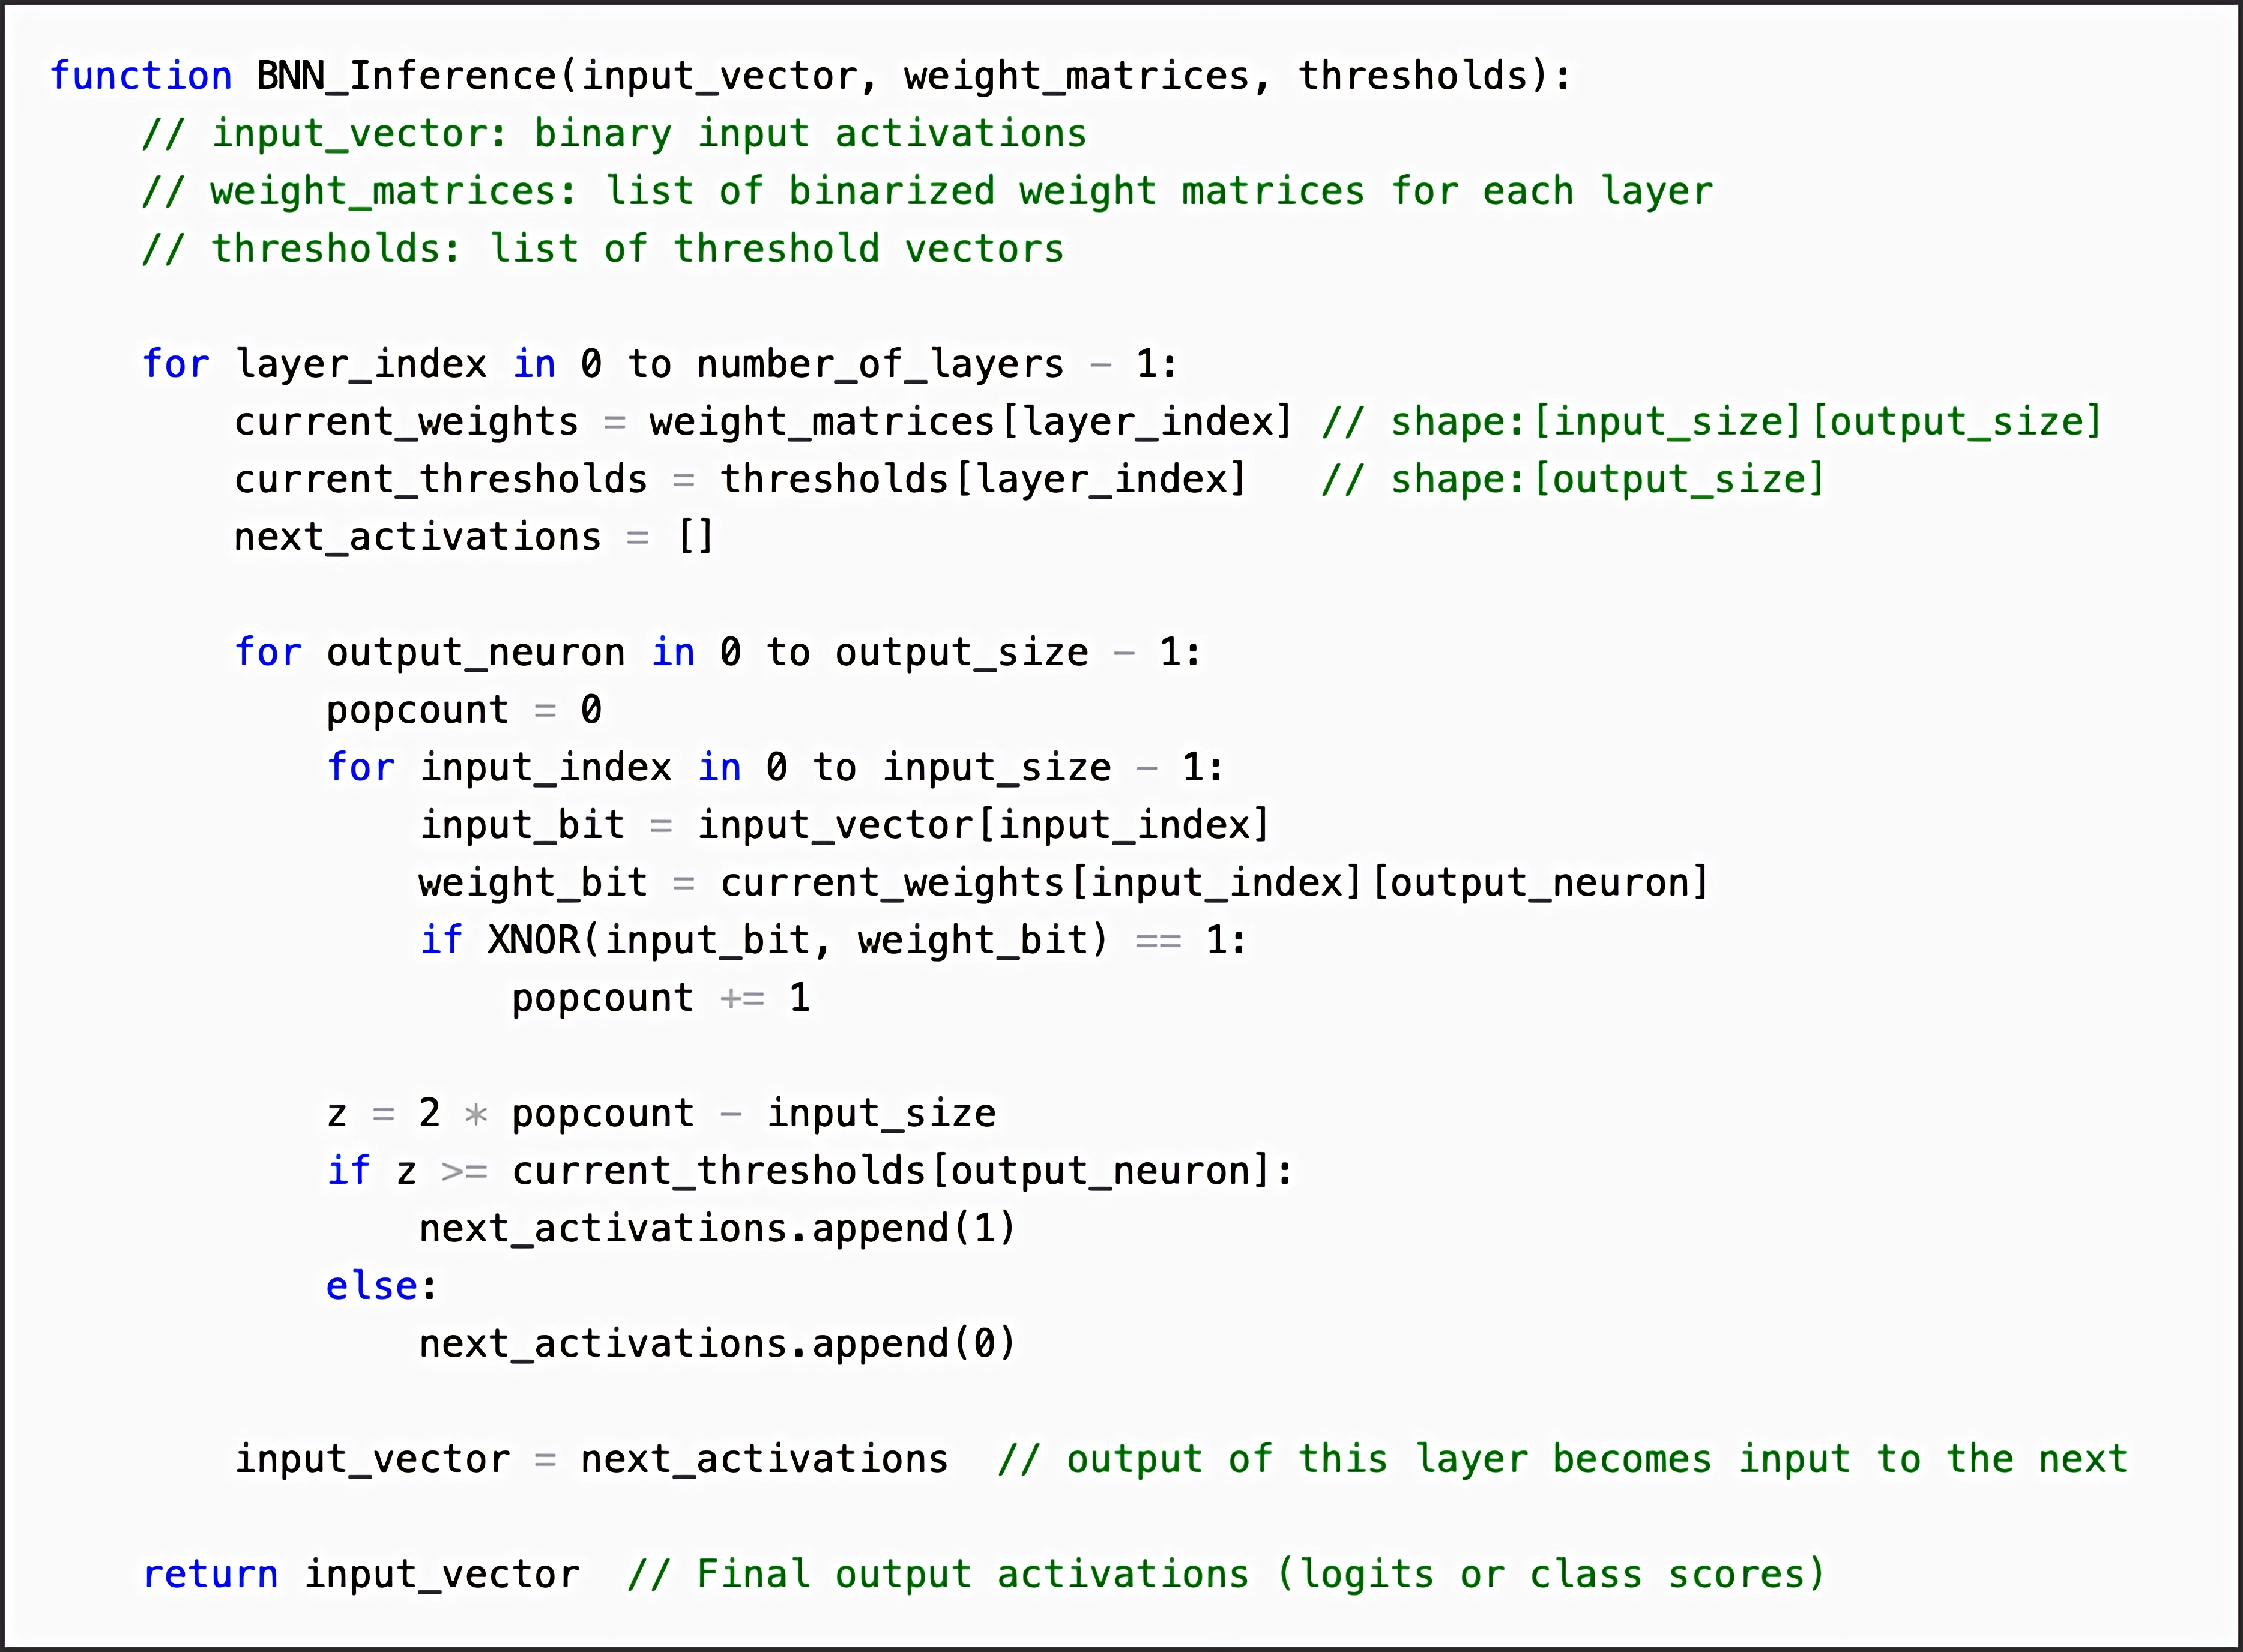
\includegraphics[width=0.95\textwidth]{figures/BNN_Inference_Pseudocode.jpg}
    \caption{Pseudocode for BNN inference using binary matrix operations and thresholds.}
    \label{fig:bnn_inference_pseudocode}
\end{figure}

\clearpage
\section{Deployment Considerations}



% CHAPTER 4 - IMPLEMENTATION
% -------------------------------------
\clearpage
\chapter{IMPLEMENTATION}
\label{chapter:implementation}
The development of the Binary Neural Network (BNN) model and its deployment onto the FPGA required a combination of software frameworks and hardware design tools, each specific to different stages of the project.

While comparative analysis was conducted across multiple levels of neuron parallelization, all implementation screenshots, synthesis reports, and power analysis results presented in this chapter correspond to the configuration using \textbf{64-level parallelism} with \textbf{dual-port BRAMs} for weight storage. This configuration was selected as the representative baseline due to its balanced trade-off between inference speed and resource utilization.

\section{Model Architecture and Training}
The Binary Neural Network (BNN) model was trained using the \textbf{TensorFlow} deep learning framework, with \textbf{Keras} as its high-level API. To support binarized operations, the \textbf{Larq} library was used. Larq extends Keras by introducing binary compatible layers and quantization-aware training capabilities, enabling both weights and activations to be reduced to 1-bit during training.

To ensure reproducibility, fixed random seeds were set for Python, NumPy and TensorFlow, keeping weight initializations consistent across training runs. The training incorporated \textbf{Quantization-Aware Training (QAT)}, allowing the network to adapt to binary constraints while preserving performance.

The model architecture consists of:
\begin{itemize}
    \item \textbf{Input Layer:} 784 features corresponding to 28$\times$28 grayscale image pixels, normalized to the range $[-1, 1]$.
    \item \textbf{First Hidden Layer:} 128 binarized neurons, fully connected to the input, followed by batch normalization.
    \item \textbf{Second Hidden Layer:} 64 binarized neurons, fully connected to the first layer, with batch normalization.
    \item \textbf{Output Layer:} 10 neurons with binarized weights but real-valued outputs, used for final argmax classification.
\end{itemize}

To improve convergence and stability, \textbf{Batch Normalization} layers were placed after each hidden and output layer. This ensures consistent feature scaling and supports threshold folding during FPGA inference.

The model is compiled using the \textbf{Adam optimizer} with an \textit{exponential learning rate decay schedule}. The learning rate starts at 0.001 and decays by a factor of 0.96 every 1000 steps using a staircase strategy. These parameters were empirically selected to achieve high accuracy while maintaining stable training.

The loss function used is \textbf{Sparse Categorical Crossentropy}, which is suitable for multi-class classification tasks with integer-labeled classes (0–9 in this case). Training was performed over \textbf{15 epochs} with a \textbf{batch size of 64}, meaning the model weights were updated after every 64 samples using mini-batch gradient descent.

The final trained model achieved a \textbf{test accuracy of 87.97\%} on the standard MNIST test set. This performance is notable given the binarization constraints and highlights the efficiency of the network architecture.

The model was saved in the \texttt{.h5} format, containing both the network weights and batch normalization statistics. This format made it straightforward to extract and convert the data for FPGA implementation.

\section{Model Export and Hardware Formatting}
After training, the weights were extracted and binarized. Each layer’s weights were thresholded and converted into 0/1 binary representations suitable for hardware implementation.

To match the memory access pattern of the FPGA, the weight matrices were transposed during export. This ensures that each row in the memory corresponds to a single neuron’s full set of weights, enabling efficient ROM access during inference.

\textbf{Batch Normalization parameters} were folded into static thresholds using the formula:
\[\theta = \left\lfloor \beta - \frac{\mu}{\sqrt{\sigma^2 + \epsilon}} \right\rceil\]
where $\beta$ is the learned offset, $\mu$ is the moving mean, $\sigma^2$ is the variance and $\epsilon$ a small constant for numerical stability. The resulting thresholds were saved as signed 11-bit integers in \texttt{.mem} files and directly loaded into ROMs in the FPGA design.


\section{Target FPGA Board}
The final hardware design was implemented on the \textbf{Nexys A7-100T FPGA Development Board} by Digilent, based on the Xilinx Artix-7 XC7A100T FPGA. This board was selected due to its large amount of logic and memory resources and ease of use with the Xilinx Vivado toolchain.

\subsection{Key specifications}
\begin{itemize}
    \item \textbf{FPGA Chip:} Xilinx Artix-7 XC7A100T-1CSG324C, providing 15,850 logic slices, each consisting of four 6-input Look-Up Tables (LUTs) and eight Flip-Flops.
    \item \textbf{Logic Resources:} 63,400 LUTs and 126,800 Flip-Flops available for combinational and sequential logic design.
    \item \textbf{Block RAM:} 4,860 Kbits of on-chip BRAM, equivalent to 135 RAMB18 blocks, used for high throughput dual-port ROMs to store model weights.
    \item \textbf{DSP Slices:} 240 DSP slices are available on the chip; however, they are not utilized in this project since the BNN relies only on bitwise XNOR and popcount operations.
    \item \textbf{Clocking:} Although the board supports internal clock speeds exceeding 450\,MHz, the design operates at a fixed frequency of 80\,MHz. This frequency was chosen to ensure reliable operation and successful timing closure during synthesis, even at higher parallelization levels.
    \item \textbf{Visual Output:} Two 4-digit seven-segment displays are used to show the final digit prediction for inference verification on hardware.
\end{itemize}
This platform provides sufficient capacity to test multiple configurations of the binary neural network, especially under varying levels of neuron parallelization.

While all simulations, synthesis and implementation steps were performed specifically targeting the Nexys A7-100T board using the Vivado Design Suite, the bitstream was not programmed onto the physical FPGA, and no on-board testing was conducted during this project.


\clearpage
\begin{table}[htbp]
    \centering
    \begin{tabular}{|c|c|p{7.5cm}|}
        \hline
        \textbf{Component} & \textbf{Tool} & \textbf{Purpose} \\
        \hline
        Training Framework & TensorFlow & Training the BNN model and managing neural network layers. \\
        \hline
        BNN Library & Larq & Provides binarized layers and quantization-aware training support. \\
        \hline
        Programming Language & Python & Used for scripting, training and weight export. \\
        \hline
        Simulation + Synthesis & Xilinx Vivado & Used for RTL design, waveform inspection, synthesis and implementation. \\
        \hline
        HDL Language & Verilog & Describes all hardware modules, FSMs, memory logic and inference pipeline. \\
        \hline
        Input/Output Medium & \texttt{.mem} Files & Store binarized weights, thresholds and test images for ROM initialization. \\
        \hline
    \end{tabular}
    \vspace{0.5\baselineskip}
    \caption{Software and Hardware Tools Used in the Project}
    \label{table:toolchain_summary}
\end{table}


\section{Hardware Architecture Overview}
The hardware design implements a feedforward BNN using a state driven control mechanism and modular memory interfaces. The inference logic processes a 28$\times$28 binarized image input through three fully connected layers.
\begin{itemize}
    \item \textbf{Input Interface:} The input image is provided as a 784-bit wire named \texttt{image}, representing the flattened 28$\times$28 grayscale image in binary form. This wire is driven by the \texttt{image\_rom} module, which retrieves preprocessed test images stored in ROM format. Each bit in \texttt{image} corresponds to a binarized pixel value, matching the structure expected by the trained BNN model.
    \item \textbf{Memory Modules:} Model weights are stored in dual-port ROMs:
    \begin{itemize}
        \item \texttt{dense\_kernel\_rom\_dualport}, which outputs to \texttt{dense\_w0[]} for Layer 1 weight access
        \item \texttt{dense\_1\_kernel\_rom\_dualport}, which outputs to \texttt{dense\_w1[]} for Layer 2 weight access
        \item \texttt{dense\_2\_kernel\_rom\_dualport}, which outputs to \texttt{dense\_w2[]} for Output Layer weight access
    \end{itemize}
    These modules are generated using \texttt{genvar} loops and enable dual-port access for two neurons per clock cycle.
    \item \textbf{Threshold ROMs:} Thresholds for the first two layers are stored in single-port LUT-based ROMs:
    \begin{itemize}
        \item \texttt{dense\_kernel\_thresholds\_rom\_lut}, which outputs to \texttt{thresh\_w0[]} for \newline Layer 1
        \item \texttt{dense\_1\_kernel\_thresholds\_rom\_lut}, which outputs to \texttt{thresh\_w1[]} for Layer 2
    \end{itemize}
    No threshold ROM is instantiated for the final layer, as its raw integer outputs are directly forwarded to the argmax comparison stage.
    \item \textbf{Output Buffers:} Intermediate layer outputs are stored in registers:
    \begin{itemize}
        \item \texttt{layer1\_out} (\texttt{reg [127:0]})
        \item \texttt{layer2\_out} (\texttt{reg [63:0]})
        \item \texttt{output\_scores} (\texttt{reg signed [9:0]} array)
    \end{itemize}
    \item \textbf{Computation Flow:} For each neuron in a layer, the module performs bitwise XNOR between input activations and stored weights, accumulates the popcount and applies a threshold to produce the next layer's activation.
    \item \textbf{Digit Output:} The predicted digit is stored in the \texttt{digit} wire after performing an argmax operation over the \texttt{output\_scores} array.
\end{itemize}
The architecture is fully parametrized using the \texttt{PARALLEL\_NEURONS} macro, which determines the number of neurons processed concurrently by instantiating parallel memory and compute logic for each layer.


\section{Finite State Machine Control}
The inference process is driven by a centralized Finite State Machine (FSM), encoded using the 3-bit registers \texttt{state} and \texttt{next\_state}. The FSM coordinates the sequential computation of each layer, accumulation of results and generation of the final predicted digit.

Each major layer computation is decomposed into a three phase sequence:
\vspace{-2em}
\begin{itemize}
    \item Row-wise XNOR operations with parallel weight fetches
    \item Popcount accumulation into \texttt{popcount[]} registers
    \item Threshold comparison to set output activations or scores
\end{itemize}
\vspace{-2em}
The FSM traverses the following five states in sequence:
\begin{enumerate}
    \item \textbf{COMPUTE\_LAYER1:}
    \begin{itemize}
        \item At each rising edge of the clock, the FSM iterates over 784 input pixels using \texttt{addr1} from 0 to 783.
        \item For each input bit, it performs bitwise XNOR with corresponding bits from \newline \texttt{dense\_w0[j][783 - addr1]} across all \texttt{PARALLEL\_NEURONS}.
        \item The XNOR result for each neuron is accumulated in \texttt{popcount[j]}.
        \item Once \texttt{addr1 == 783}, \texttt{process\_neuron1} is set to 1 in the next cycle, indicating all inputs are processed for this neuron group.
        \item Then, $z_j = 2 \cdot \texttt{popcount[j]} - 784$ is computed and stored in \texttt{z[j]} when \texttt{z\_ready == 0}, after which \texttt{z\_ready} is set to 1.
        \item Threshold comparison is performed: if $z_j \geq \texttt{thresh\_w0[j]}$, then \newline \texttt{layer1\_out[neuron\_idx1 + j]} is set to 1; otherwise 0.
        \item After activation, \texttt{addr1}, \texttt{z\_ready}, \texttt{process\_neuron1}, and all \texttt{popcount[j]} are reset for the next neuron batch.
        \item \texttt{neuron\_idx1}, which tracks the starting index of the current neuron group being processed, is incremented by \texttt{PARALLEL\_NEURONS}. When all neurons in Layer 1 are processed (\texttt{neuron\_idx1 >= 128 - PARALLEL\_NEURONS}), \texttt{done\_layer1} is set to 1.
    \end{itemize}

    \item \textbf{COMPUTE\_LAYER2:}
    \begin{itemize}
        \item \texttt{addr2} loops over Layer 1 outputs from \texttt{layer1\_out[addr2]} for indices 0 to 127.
        \item At each step, XNOR is computed with \texttt{dense\_w1[j][127 - addr2]}, and results are accumulated in \texttt{popcount[j]}.
        \item When \texttt{addr2 == 127}, \texttt{process\_neuron2} is raised in the next cycle. Then \newline $z_j = 2 \cdot \texttt{popcount[j]} - 128$ is calculated and stored into \texttt{z[j]}.
        \item The activation result is written to \texttt{layer2\_out[neuron\_idx2 + j]} by comparing with \texttt{thresh\_w1[j]}.
        \item After activation, \texttt{addr2}, \texttt{z\_ready}, \texttt{process\_neuron2}, and all \texttt{popcount[j]} are reset for the next neuron batch.
        \item \texttt{neuron\_idx2} is incremented by \texttt{PARALLEL\_NEURONS}. When all neurons in Layer 2 are processed (\texttt{neuron\_idx2 >= 64 - PARALLEL\_NEURONS}), \texttt{done\_layer2} is set to 1.
    \end{itemize}
    
    \item \textbf{COMPUTE\_OUTPUT:}
    \begin{itemize}
        \item \texttt{addr3} loops over Layer 2 outputs from \texttt{layer2\_out[addr3} for indices 0 to 63.
        \item Performs XNOR with weights \texttt{dense\_w2[j][63 - addr3]} and accumulates in \texttt{popcount[j]}.
        \item Once \texttt{addr3 == 63}, \texttt{process\_neuron3} is set and in the next cycle, \newline $z_j = 2 \cdot \texttt{popcount[j]} - 64$ is evaluated.
        \item Unlike previous layers, no thresholding is applied. The raw $z_j$ values are stored directly in \texttt{output\_scores[neuron\_idx3 + j]}.
        \item Following this, \texttt{addr3}, \texttt{z\_ready}, \texttt{process\_neuron3}, and \texttt{popcount[j]} are reset for the next neuron batch and \texttt{neuron\_idx3} increments by \texttt{PARALLEL\_NEURONS}.
        \item When \texttt{neuron\_idx3 >= 10 - PARALLEL\_NEURONS}, \texttt{done\_output} is set.
    \end{itemize}

    \item \textbf{ARGMAX\_OUTPUT:}
    \begin{itemize}
        \item Begins by initializing \texttt{temp\_max = output\_scores[0]} and \texttt{temp\_index = 0}, with \texttt{compare\_idx = 1}.
        \item At each clock cycle, compares \texttt{output\_scores[compare\_idx]} against \newline \texttt{temp\_max}, updating both if a larger value is found.
        \item Increments \texttt{compare\_idx} until it reaches 9. Then, stores the index of the maximum score in \texttt{predicted\_digit}.
        \item Asserts \texttt{done\_argmax = 1} and clears \texttt{argmax\_started}.
    \end{itemize}

    \item \textbf{DONE:}
    \begin{itemize}
        \item No computation is performed.
        \item The output signal \texttt{done} is held high indefinitely.
        \item FSM remains in this state until \texttt{reset} is reasserted.
    \end{itemize}
\end{enumerate}


\section{Parametrization and Scalability}
The design supports configurability of parallelism and neuron counts using Verilog parameters:
\begin{itemize}
    \item \texttt{parameter PARALLEL\_NEURONS} defines how many neurons are processed in parallel in each batch.
    \item Threshold and weight ROM instantiations are generated using \texttt{genvar} blocks based on this parameter.
    \item Internally, \texttt{neuron\_idx1}, \texttt{neuron\_idx2}, and \texttt{neuron\_idx3} traverse the neuron space in increments of \texttt{PARALLEL\_NEURONS}, supporting batch processing.
\end{itemize}
Scalability is observed at synthesis time by adjusting the \texttt{PARALLEL\_NEURONS} value. Inference time decreases with higher parallelization, but resource usage, especially BRAMs, increases proportionally. The design uses falls back to LUT-based ROMs when BRAM resources are exhausted (automatically handled by Vivado).


\section{Module Descriptions}
The Verilog design follows a hierarchical structure. Each hardware block encapsulates a specific functionality, enabling clean separation between computation, memory access, input feeding and output display. The overall module hierarchy is as follows:
\begin{itemize}
    \item \textbf{\texttt{bnn\_top.v}} \textit{(Top-Level Module)}
    \begin{itemize}
        \item Instantiates and connects the following components:
        \begin{itemize}
            \item[\textperiodcentered] \texttt{bnn\_inference}: Core inference logic
            \item[\textperiodcentered] \texttt{image\_rom}: Provides the binary input image
            \item[\textperiodcentered] \texttt{seven\_segment\_decoder}: Displays the output digit
        \end{itemize}
        \item Handles reset, clock and port wiring
    \end{itemize}
    \item \textbf{\texttt{bnn\_inference.v}} \textit{(Inference Core)}
    \begin{itemize}
        \item Implements the main finite state machine for controlling inference flow
        \item Contains:
        \begin{itemize}
            \item[\textperiodcentered] Parallel XNOR-popcount logic for binary matrix operations
            \item[\textperiodcentered] Threshold comparison and binary activation per neuron
            \item[\textperiodcentered] Argmax logic to select the final prediction
        \end{itemize}
        \item Interfaces with weight and threshold ROM modules using address signals and memory fetch wires
    \end{itemize}
    \item \textbf{\texttt{model\_rom.v}} \textit{(Central ROM Module for All Weights and Thresholds)}
    \begin{itemize}
        \item Includes three dual-port BRAM based ROM modules:
        \begin{itemize}
            \item[\textperiodcentered] \texttt{dense\_kernel\_rom\_dualport.v}: Layer 1 weights (\texttt{dense\_w0[]})
            \item[\textperiodcentered] \texttt{dense\_1\_kernel\_rom\_dualport.v}: Layer 2 weights (\texttt{dense\_w1[]})
            \item[\textperiodcentered] \texttt{dense\_2\_kernel\_rom\_dualport.v}: Output layer weights (\texttt{dense\_w2[]})
        \end{itemize}
        \item Also includes:
        \begin{itemize}
            \item[\textperiodcentered] \texttt{dense\_kernel\_thresholds\_rom\_lut.v}: Layer 1 thresholds (\texttt{thresh\_w0[]})
            \item[\textperiodcentered] \texttt{dense\_1\_kernel\_thresholds\_rom\_lut.v}: Layer 2 thresholds (\texttt{thresh\_w1[]})
        \end{itemize}
        \item No threshold ROM is used for the output layer since it outputs raw scores for argmax
    \end{itemize}
    \item \textbf{\texttt{image\_rom.v}} \textit{(Input Image Memory)}
    \begin{itemize}
        \item Stores a single binary encoded 28$\times$28 image (784 bits) as \texttt{image[783:0]}
        \item Image is initialized from an external \texttt{.mem} file
        \item Used exclusively for simulation and synthesis-time preload; real-time image loading is not supported in the current design
    \end{itemize}
    \item \textbf{\texttt{seven\_segment\_decoder.v}} \textit{(Display Interface)}
    \begin{itemize}
        \item Converts the 4-bit \texttt{digit} output into control signals for 7-segment displays
        \item Outputs a 7-bit vector (\texttt{segments}) corresponding to the numerical digit pattern
        \item Used for visual verification of inference results on hardware
    \end{itemize}
\end{itemize}
All modules interact through well-defined data and control paths managed at the \texttt{bnn\_top} level, allowing a scalable and verifiable design structure.

\clearpage
\section{Simulation, Synthesis and Implementation}
The complete hardware flow was executed using the \textbf{Xilinx Vivado Design Suite}, encompassing simulation, synthesis, implementation and power analysis stages. Each stage was carefully evaluated to ensure the design met functional correctness, resource efficiency and timing closure targets for the selected FPGA platform.

\subsection{Simulation and Verification}
The inference design was verified using behavioral simulation in Vivado. Testbenches provided input to the \texttt{bnn\_top} module, with pre-loaded \texttt{.mem} files supplying the input image, weights and thresholds. Waveform inspection via \texttt{.vcd} files allowed cycle-level monitoring of internal signals.

Correctness was evaluated by comparing the output digit predictions against those generated by the original Python trained model. Intermediate outputs like \texttt{layer1\_out}, \texttt{layer2\_out} and \texttt{output\_scores[]} were manually cross-checked to ensure alignment at each stage.

Figure~\ref{fig:sim_waveform} illustrates a waveform captured during simulation, showing the inference flow for a sample image. Key signals such as FSM state transitions, neuron indices, intermediate activations and the final predicted digit (\texttt{digit = 3}) can be observed, verifying functional correctness throughout all computation phases.

\begin{figure}[H]
    \centering
    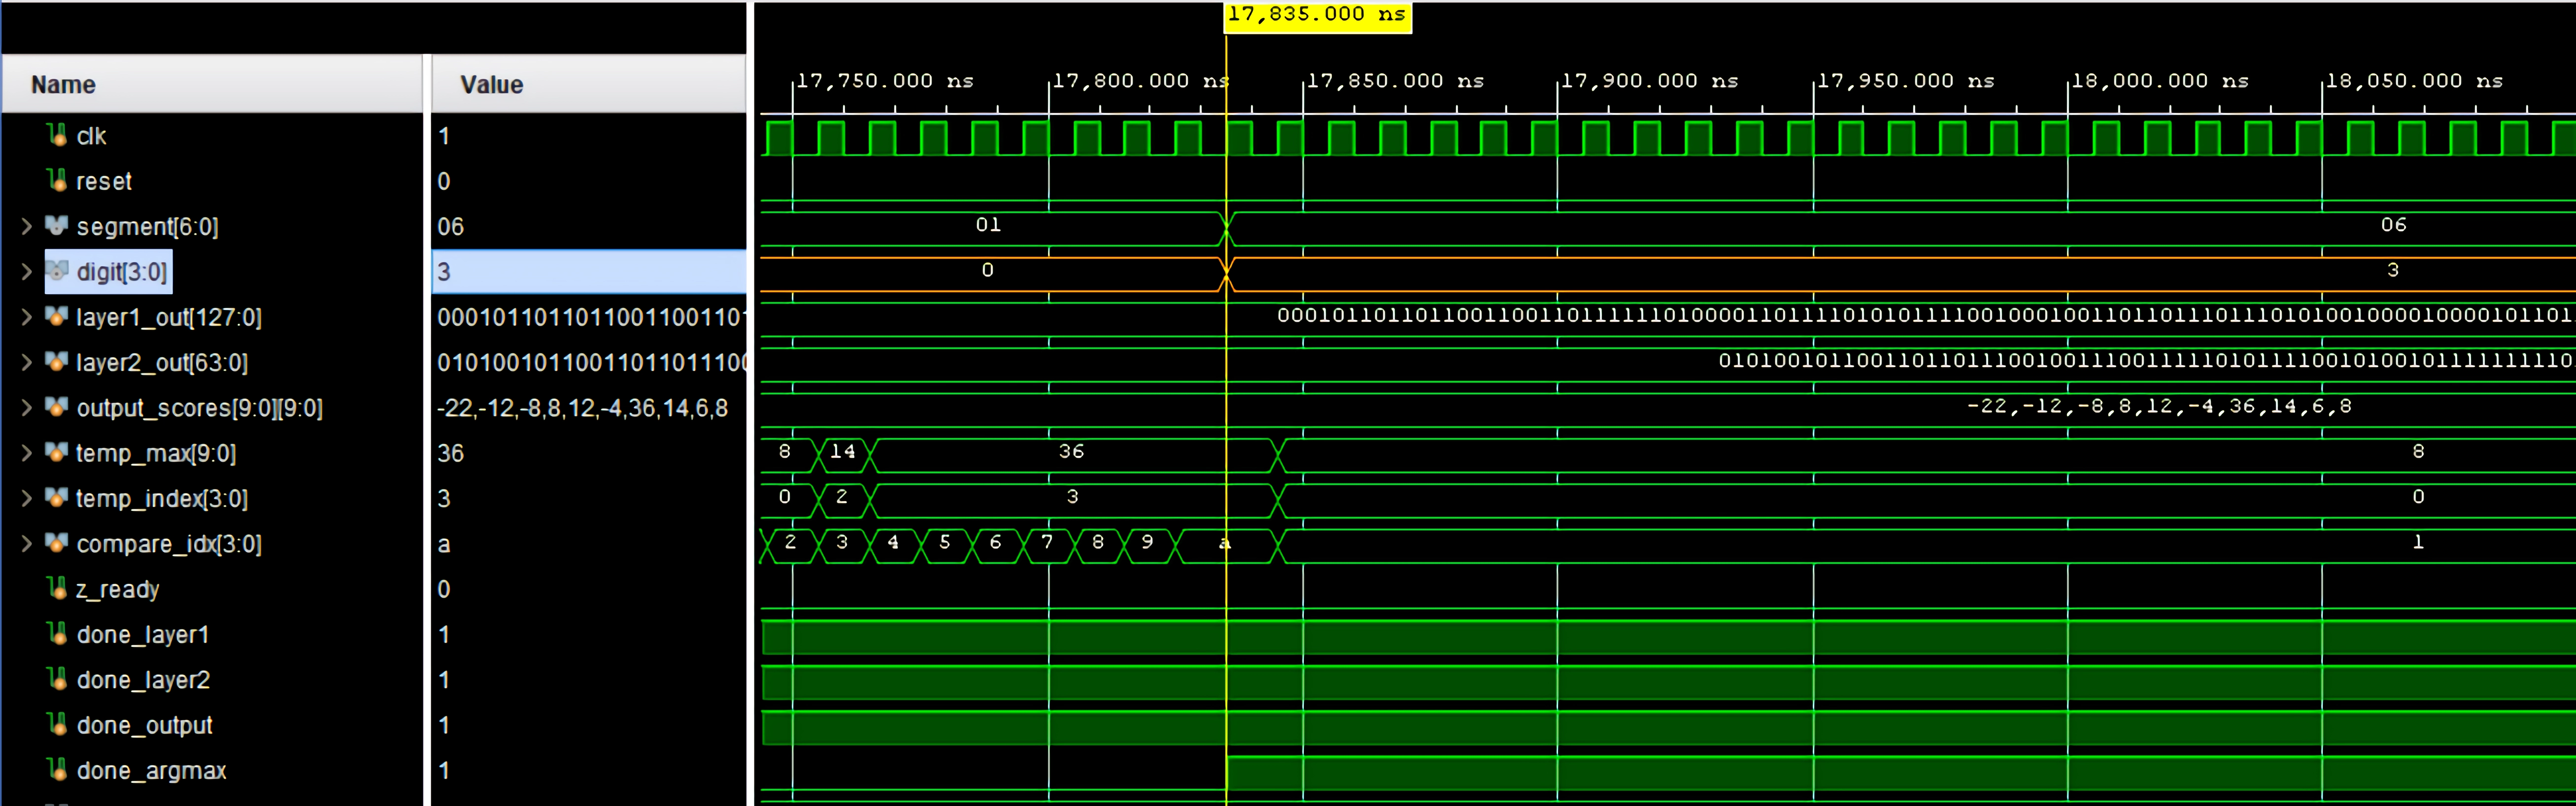
\includegraphics[width=\textwidth]{simulation_waveform_level_64_cropped(digit 3).png}
    \caption{Simulation waveform of BNN inference with digit prediction = 3.}
    \label{fig:sim_waveform}
\end{figure}

\clearpage
\subsection{RTL Synthesis}
Vivado's RTL Synthesis engine translated the Verilog source into a gate-level netlist customized for the Artix-7 XC7A100T architecture. This process was performed after verifying the functionality of all modules through behavioral simulation. The synthesis process included HDL parsing, optimization of logic expressions and mapping to specific hardware primitives such as LUTs, Flip-Flops and BRAMs.

Resource utilization results were extracted for the design configured at \texttt{PARALLEL\_NEURONS = 64}, with dual-port BRAMs used for weight storage. The key goals of synthesis were to:
\begin{itemize}
    \item Evaluating logic resource usage including Look-Up Tables (LUTs), Flip-Flops (FFs), BRAMs and I/O buffers
    \item Verifying the proper instantiation of memory modules, FSM logic and datapath structures
    \item Ensuring synthesis passes without critical warnings, confirming structural correctness
\end{itemize}
Figure~\ref{fig:synth_schematic} shows the synthesized RTL schematic of the top-level module. The design is flattened into its post-synthesis netlist, with the \texttt{bnn\_inference} core module interfaced with I/O buffers and key internal registers. This view confirms correct synthesis and routing of major signal paths, including clock, reset and digit display.
\begin{figure}[H]
    \centering
    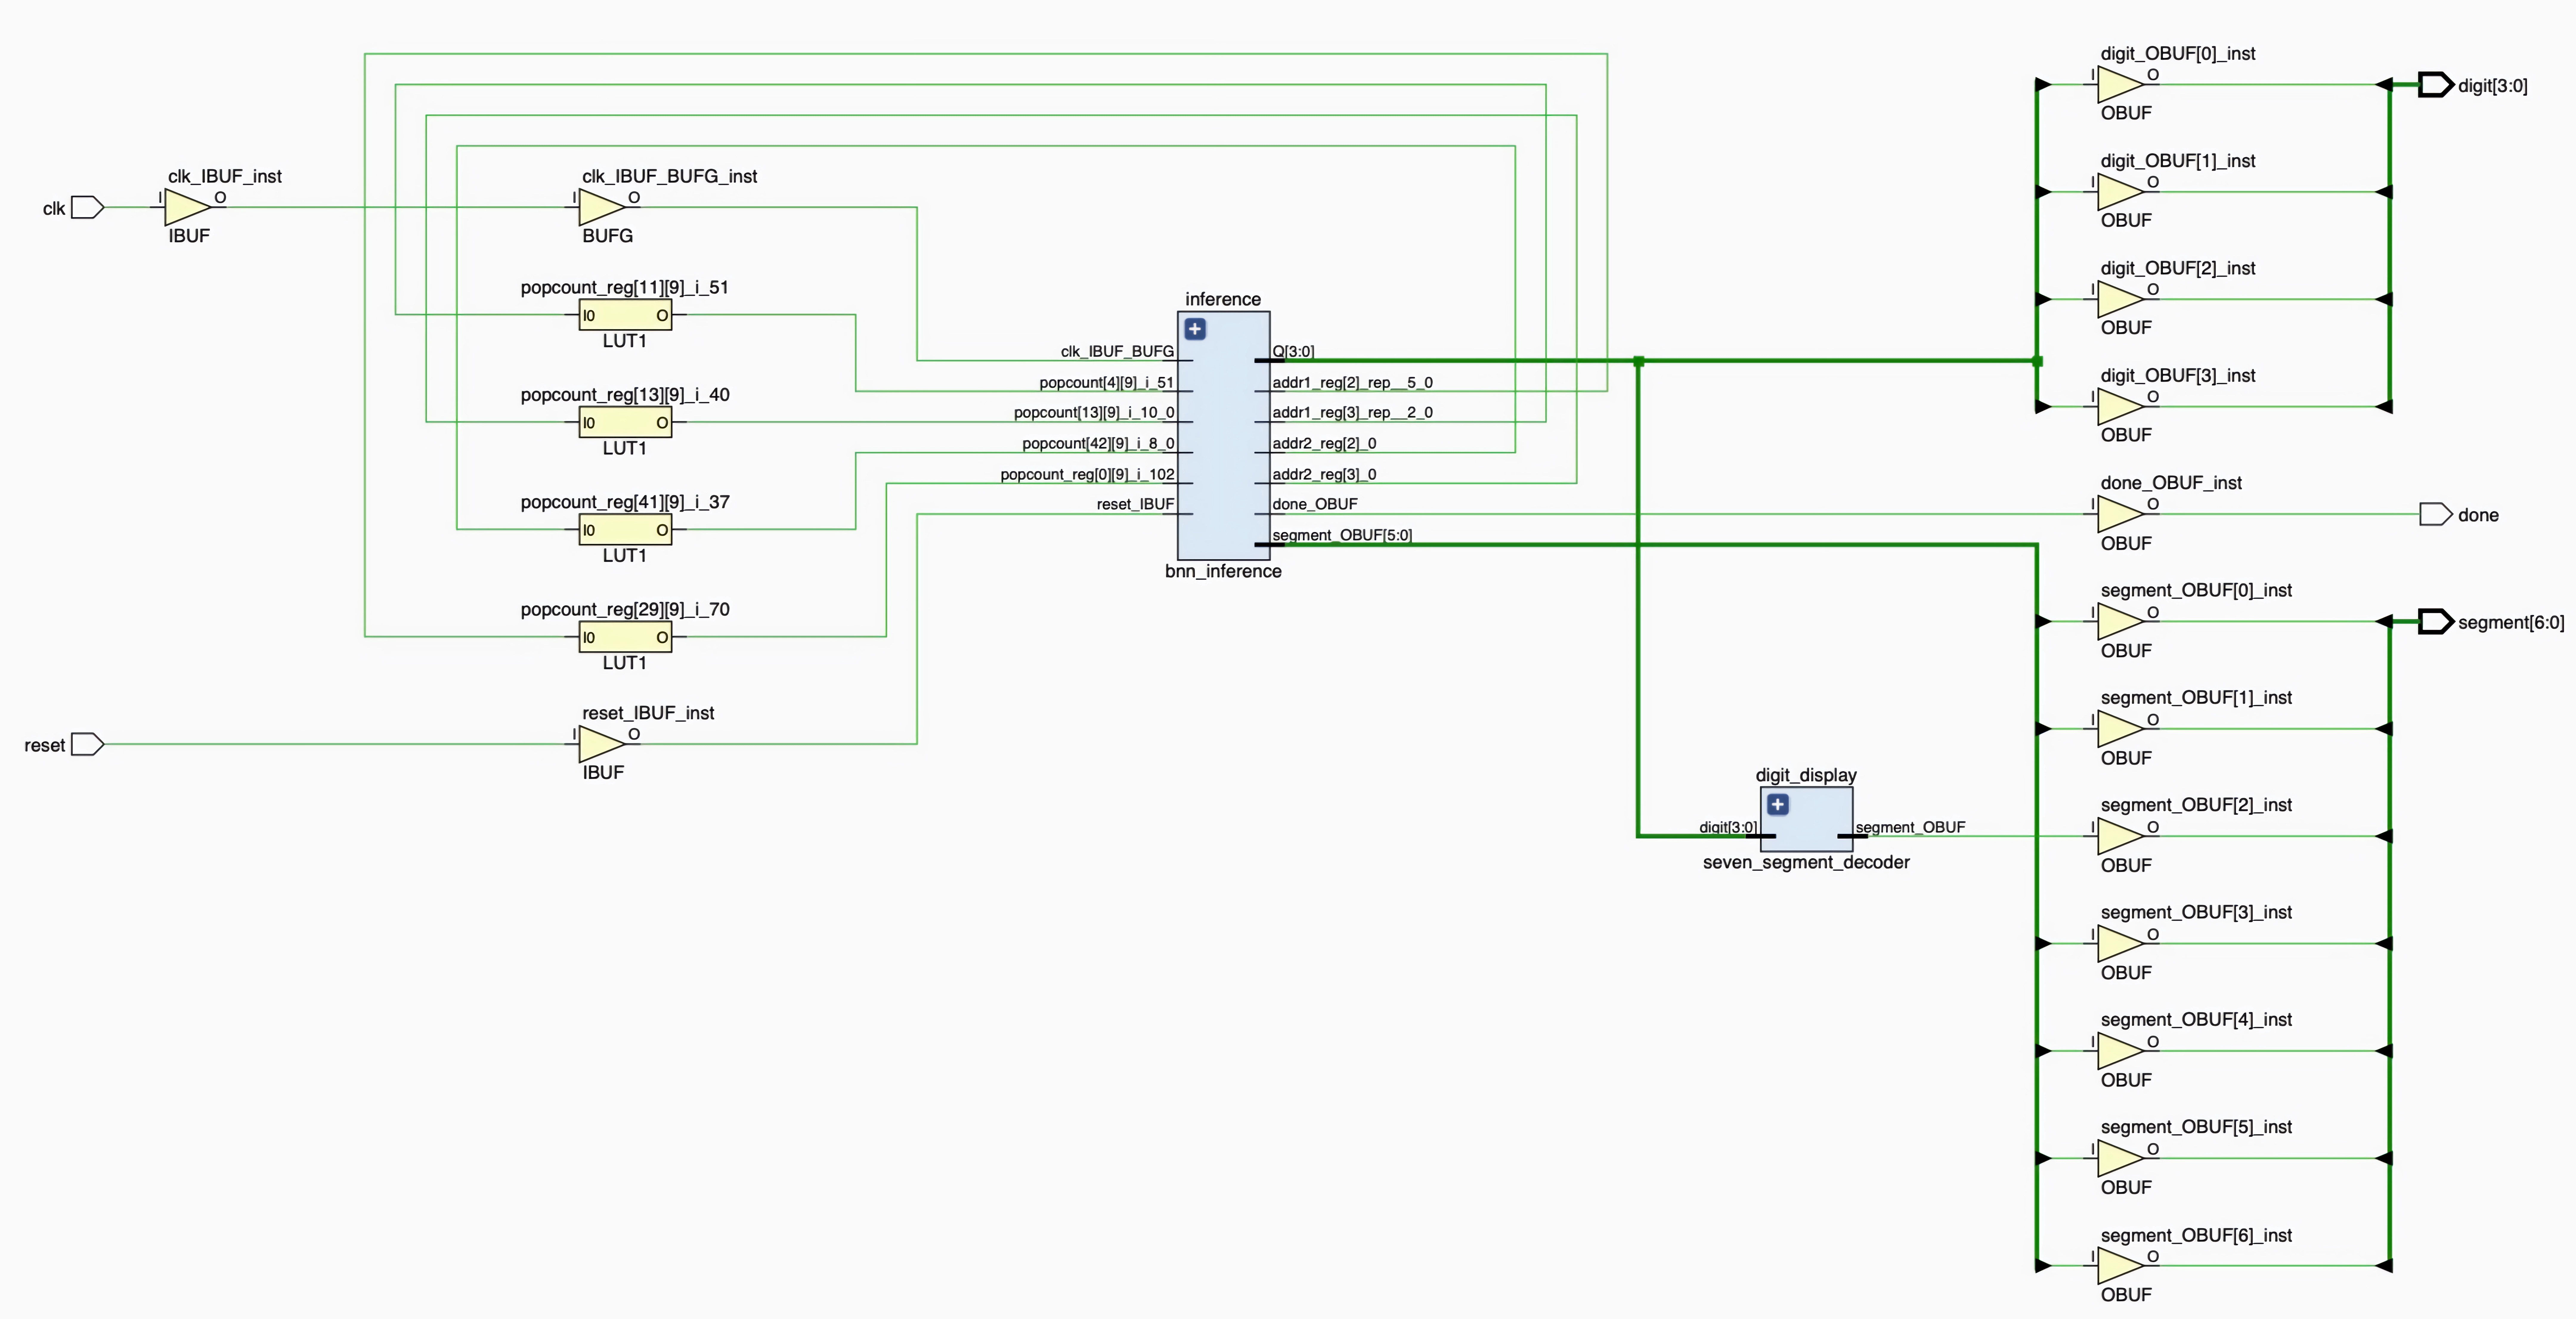
\includegraphics[width=\textwidth]{schematic_level_64(synthesis).jpeg}
    \caption{Synthesized schematic view for the top-level module at 64-parallel configuration.}
    \label{fig:synth_schematic}
\end{figure}

To confirm correctness and visualize the design hierarchy, Figure~\ref{fig:elab_rtl} shows the elaborated RTL netlist generated before synthesis. This view confirms that all submodules were instantiated as expected.

\begin{figure}[H]
    \centering
    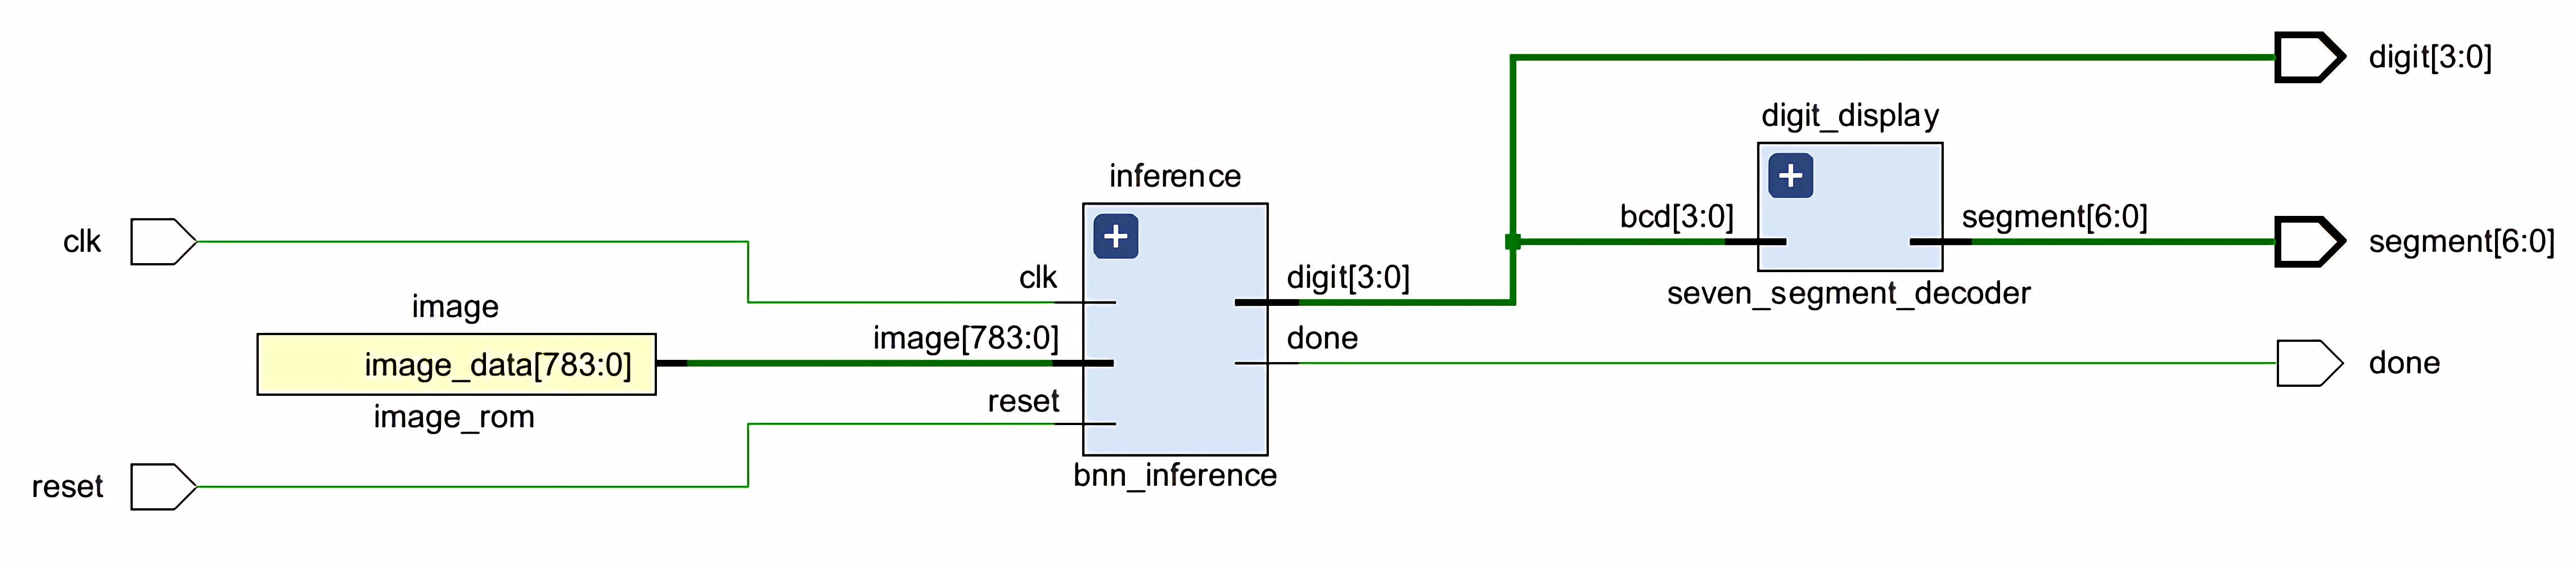
\includegraphics[width=\textwidth]{elaborated_design_level_64_(rtl_analysis).png}
    \caption{Elaborated RTL netlist prior to synthesis, confirming structural hierarchy.}
    \label{fig:elab_rtl}
\end{figure}

These synthesis results validated that the design was structurally sound and resource-efficient given the project constraints and formed the baseline for implementation and power analysis.

\subsection{Post-Synthesis Implementation}
Following synthesis, the design was passed through Vivado's physical implementation stages, which includes logic optimization, placement and routing across the FPGA fabric. This stage maps logical blocks to specific physical resources while optimizing for timing and congestion.
\subsubsection{Timing Verification} \hfill\\
Vivado's implementation tools ensured that all constraints for clock timing, signal integrity and interconnect delay were satisfied. The implementation process addressed the following:
\begin{itemize}
    \item Ensuring setup and hold timing requirements were met across all paths for the 80\,MHz system clock.
    \item Eliminating any critical path violations by adjusting placement and routing.
    \item Managing BRAM usage and interconnect congestion, especially under high parallelism (\texttt{PARALLEL\_NEURONS = 64}).
\end{itemize}

Post-implementation timing was verified using Vivado's static timing analyzer. The design achieved zero timing violations, with all slack margins reported as positive. Figure~\ref{fig:timing_summary} summarizes the setup, hold and pulse width timing results.

\begin{figure}[H]
    \centering
    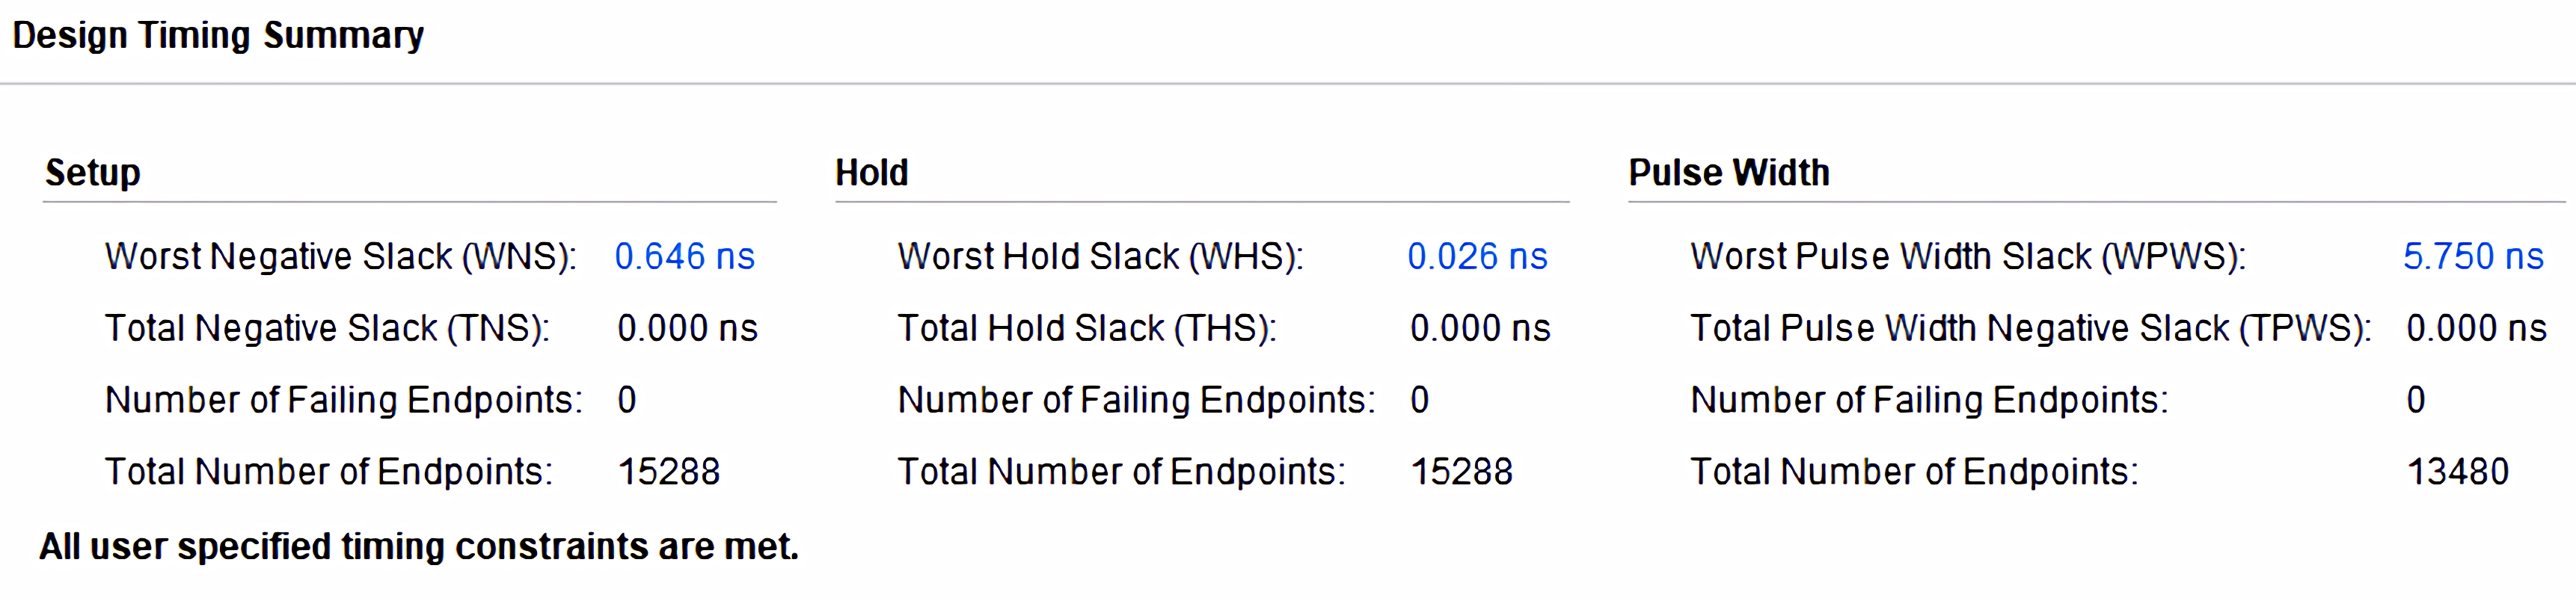
\includegraphics[width=0.9\textwidth]{timing_summary_level_64(implementation).png}
    \caption{Timing summary confirming successful closure at 80\,MHz.}
    \label{fig:timing_summary}
\end{figure}
In the setup section, the \textbf{Worst Negative Slack (WNS)} is 0.646\,ns, meaning that the critical path is within acceptable limits with positive slack, satisfying setup timing constraints. For hold timing, the \textbf{Worst Hold Slack (WHS)} is 0.026\,ns, indicating that no hold violations are present. The pulse width check shows a \textbf{Worst Pulse Width Slack (WPWS)} of 5.750\,ns, confirming that all signals maintain sufficient high or low durations to ensure reliable operation. With zero negative slack and zero failing endpoints across all checks, the design is fully timing safe at the target frequency of 80\,MHz.
\subsubsection{Resource Utilization Summary} \hfill\\
Figure~\ref{fig:resource_utilization} presents the post-implementation \textbf{resource utilization report} for the design configured with \texttt{PARALLEL\_NEURONS = 64}. The utilization summary indicates that 16,629 of the 63,400 available LUTs were used, corresponding to 26.23\% of the total logic capacity. This reflects the logic needed for operations like XNOR and popcount, controlling the FSM and generating addresses for memory access in each layer."

In terms of sequential resources, the design utilizes 13,215 out of 126,800 flip-flops (10.42\%), which shows that despite the design's complexity, the usage remains comfortably within device limits.

Notably, the most heavily consumed resource is  Block RAM. A total of 132 out of 135 BRAM blocks are used, reaching a utilization of 97.78\%. This high percentage is expected due to several large dual-port ROMs instantiated for storing weights and thresholds across the three layers of the BNN. The aggressive parallelization further increases BRAM usage, as more ROM blocks are instantiated to support concurrent access.

Lastly, only 14 out of 210 general purpose I/O ports (6.67\%) are utilized. These are dedicated to interfacing with the clock, reset, 7-segment display output and debugging interfaces.

This breakdown shows that the design fits well within the XC7A100T’s resources for LUTs and flip-flops, but comes close to the BRAM limit. This was a necessary tradeoff to achieve faster processing with wide memory access.

\begin{figure}[H]
    \centering
    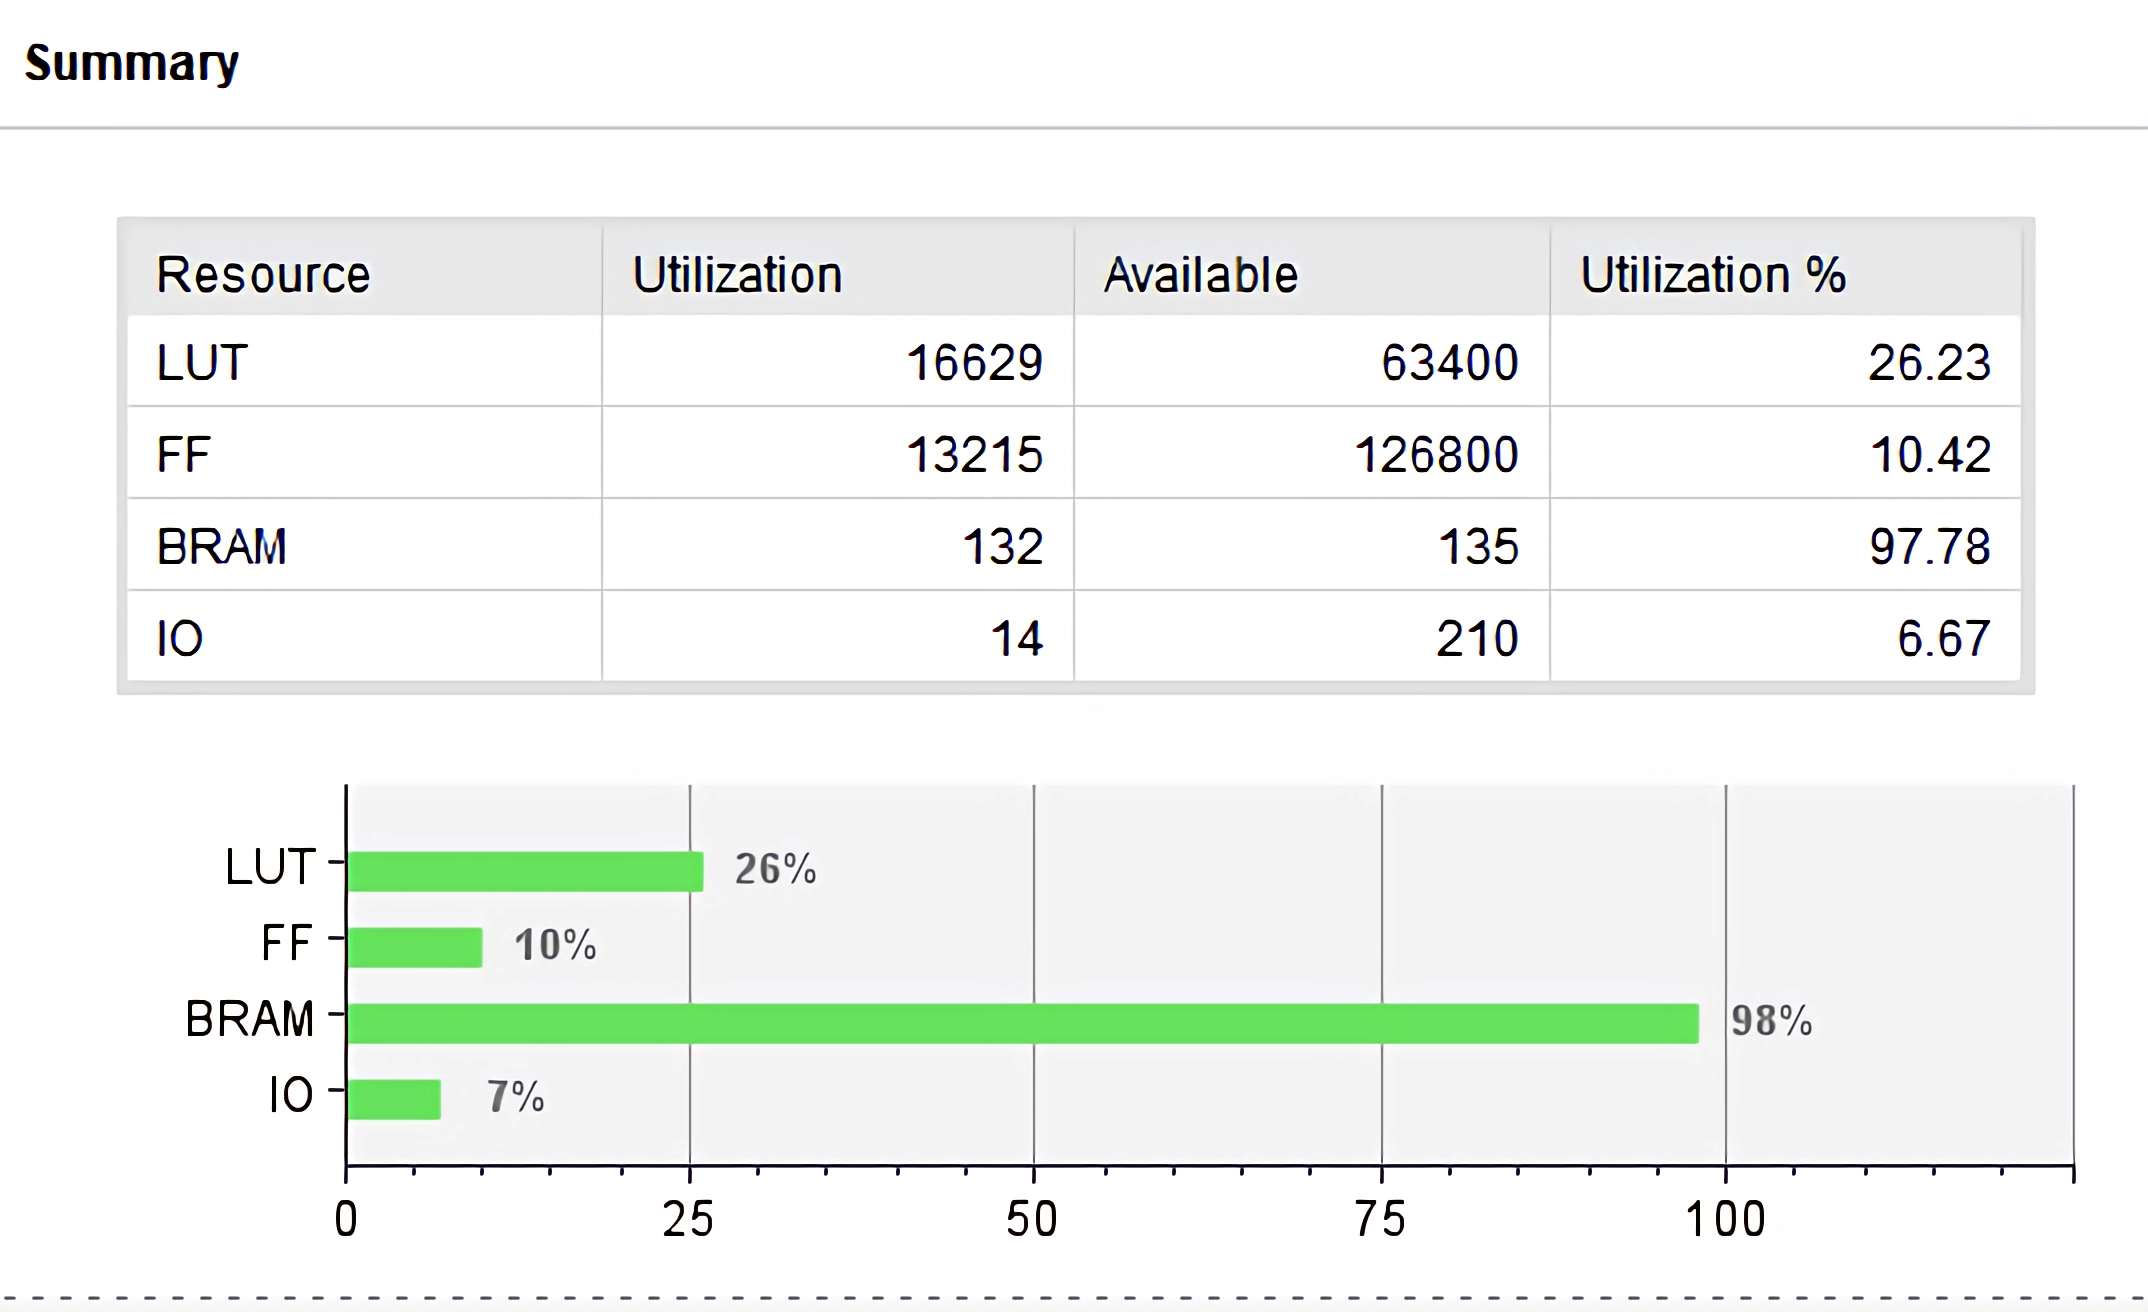
\includegraphics[width=0.6\textwidth]{resource_utilization_level_64(implementation).png}
    \caption{Post-implementation resource utilization for \texttt{PARALLEL\_NEURONS = 64}.}
    \label{fig:resource_utilization}
\end{figure}


\subsection{Power Analysis}
Vivado’s Power Analyzer was used after implementation to estimate the power consumption of the design. This analysis is based on actual signal activity from the post-place-and-route netlist. Both static (leakage) and dynamic (switching) power components were included.

As shown in Figure~\ref{fig:power_analysis}, the total estimated on-chip power is approximately \textbf{0.617,W}. Of this, \textbf{0.512,W} (83\%) is dynamic power and \textbf{0.105,W} (17\%) is static. The high dynamic power usage is mostly due to the extensive use of BRAM, which alone accounts for \textbf{0.376,W} or 74\% of the total dynamic power.

Other contributors to dynamic power include:
\vspace{-2em}
\begin{itemize}
    \item Clocks: \textbf{0.056,W} (11\%)
    \item Signals: \textbf{0.040,W} (8\%)
    \item Logic (LUTs/Flip-Flops): \textbf{0.039,W} (8\%)
    \item I/O: \textbf{0.001,W} (negligible)
\end{itemize}
\vspace{-2em}
The high BRAM consumption reflects the design’s memory-intensive architecture. Since a large number of dual-port ROMs are used to support parallel neuron access, the overall memory switching activity is high. This is the main source of dynamic power.

The junction temperature is reported as \textbf{27.8\textdegree C}, with a thermal margin of over \textbf{57\textdegree C}, indicating that the chip operates well within safe thermal limits. This ensures that the design remains stable and does not require additional cooling measures under typical conditions.

\begin{figure}[H]
    \centering
    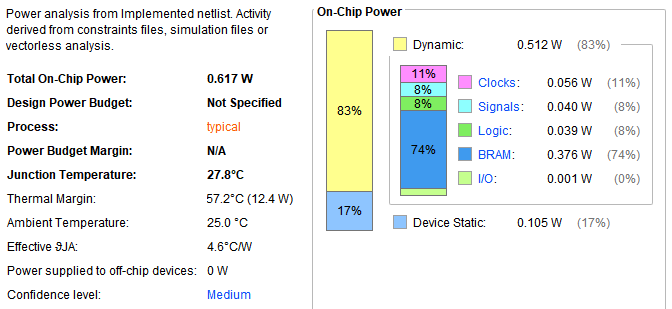
\includegraphics[width=0.8\textwidth]{power_consumption_level 64(implementation).png}
    \caption{Post-implementation power consumption breakdown for 64-level parallelization.}
    \label{fig:power_analysis}
\end{figure}

The moderate total power consumption means that the design is suitable for deployment on mid-range FPGAs like the Artix-7 without exceeding thermal or power budgets. However, the high BRAM usage and associated power cost imply that any scaling of the design (increasing parallelism) may require a higher-end FPGA with more power headroom and memory resources. This affects not only energy efficiency but also system cost, as higher-capacity devices generally come with increased price and board complexity.

\subsection{Summary}
The entire workflow, from simulation to hardware mapping, ensured that the Binary Neural Network implementation remained functionally correct, resource efficient and compliant with timing and power constraints. Although the design was not deployed to the physical board, the results validate its readiness for hardware deployment.


% CHAPTER 5 - TEST & RESULTS
\clearpage
\chapter{TEST \& RESULTS}
\label{chapter:test_and_results}

\section{Testing Methodology}
All testing was performed using Vivado 2024.1, targeting the Xilinx Artix-7 XC7A100T FPGA. Functional and timing correctness were evaluated using testbenches, with \texttt{.mem} files providing binarized weights, thresholds and MNIST test images. These files were loaded into ROM modules at simulation start.

The \texttt{bnn\_top\_tb} testbench applied clock/reset signals and observed the \texttt{digit} and \texttt{done} outputs. Waveform viewers and simulation logs were used to monitor FSM transitions, intermediate layer outputs and final predictions.

Correctness was validated by comparing predicted digits against CPU-based inference results from the trained Python model. Tests were repeated across parallelization levels and memory configurations (BRAM vs LUT) to enable detailed performance comparisons.

\section{Correctness Verification}
To validate the correctness of the hardware implementation, a total of 100 binarized MNIST test images were evaluated on the FPGA design, with 10 unique images for each digit from 0 to 9. These images were converted into \texttt{.mem} files and fed into the design one by one, while the predicted digit was recorded after each simulation.

The resulting predictions were compared against the expected digit labels. Out of 100 test cases, 87 were classified correctly, resulting in an overall accuracy of \textbf{87\%}. This is highly consistent with the trained software model's test accuracy of \textbf{87.97\%}, confirming that the quantized model behavior has been accurately replicated on hardware.

Table~\ref{table:confusion_matrix_fpga} shows the confusion matrix summarizing the predictions. Each row represents the true label, and each column represents the predicted digit. Correct predictions are located on the diagonal and highlighted in green, while incorrect classifications appear off-diagonal in red.

\begin{table}[H]
\centering
\renewcommand{\arraystretch}{1.2}
\makebox[\textwidth][c]{%
\begin{tabular}{
    |c||
    >{\centering\arraybackslash}p{0.85cm}|
    >{\centering\arraybackslash}p{0.85cm}|
    >{\centering\arraybackslash}p{0.85cm}|
    >{\centering\arraybackslash}p{0.85cm}|
    >{\centering\arraybackslash}p{0.85cm}|
    >{\centering\arraybackslash}p{0.85cm}|
    >{\centering\arraybackslash}p{0.85cm}|
    >{\centering\arraybackslash}p{0.85cm}|
    >{\centering\arraybackslash}p{0.85cm}|
    >{\centering\arraybackslash}p{0.85cm}|
}
    \hline
    \textbf{True$\setminus$Pred} & \textbf{0} & \textbf{1} & \textbf{2} & \textbf{3} & \textbf{4} & \textbf{5} & \textbf{6} & \textbf{7} & \textbf{8} & \textbf{9} \\
    \hline\hline
    \textbf{0} & \textcolor{green!50!black}{10} & 0 & 0 & 0 & 0 & 0 & 0 & 0 & 0 & 0 \\
    \hline
    \textbf{1} & 0 & \textcolor{green!50!black}{9} & 0 & \textcolor{red!90!black}{1} & 0 & 0 & 0 & 0 & 0 & 0 \\
    \hline
    \textbf{2} & \textcolor{red!90!black}{3} & 0 & \textcolor{green!50!black}{6} & 0 & 0 & 0 & 0 & \textcolor{red!90!black}{1} & 0 & 0 \\
    \hline
    \textbf{3} & 0 & 0 & \textcolor{red!90!black}{1} & \textcolor{green!50!black}{9} & 0 & 0 & 0 & 0 & 0 & 0 \\
    \hline
    \textbf{4} & \textcolor{red!90!black}{1} & 0 & 0 & 0 & \textcolor{green!50!black}{8} & 0 & 0 & 0 & \textcolor{red!90!black}{1} & 0 \\
    \hline
    \textbf{5} & 0 & 0 & 0 & \textcolor{red!90!black}{1} & \textcolor{red!90!black}{1} & \textcolor{green!50!black}{8} & 0 & 0 & 0 & 0 \\
    \hline
    \textbf{6} & \textcolor{red!90!black}{1} & 0 & \textcolor{red!90!black}{1} & 0 & 0 & 0 & \textcolor{green!50!black}{8} & 0 & 0 & 0 \\
    \hline
    \textbf{7} & \textcolor{red!90!black}{1} & 0 & 0 & 0 & 0 & 0 & 0 & \textcolor{green!50!black}{9} & 0 & 0 \\
    \hline
    \textbf{8} & 0 & 0 & 0 & 0 & 0 & 0 & 0 & 0 & \textcolor{green!50!black}{10} & 0 \\
    \hline
    \textbf{9} & 0 & 0 & 0 & 0 & \textcolor{red!90!black}{1} & 0 & 0 & \textcolor{red!90!black}{2} & 0 & \textcolor{green!50!black}{7} \\
    \hline
\end{tabular}
}
\vspace{1em}
\caption{Confusion matrix of FPGA predictions on 100 test images}
\label{table:confusion_matrix_fpga}
\end{table}


\section{Speed vs Resource Trade-Off Results}
To evaluate the scalability of the design, thirteen hardware configurations were tested by varying the \texttt{PARALLEL\_NEURONS} parameter from 1 to 128. For each configuration up to and including 64-level parallelism, two versions were synthesized: one using dual-port BRAMs for weight storage and one using LUT based ROMs. At 128-level parallelism, BRAM capacity is fully exhausted, and partial fallback is no longer possible, so only the LUT based version could be synthesized. All timing, power and resource utilization results were taken from post-implementation reports in Vivado.


\subsection{Latency Comparison}
As shown in Table~\ref{table:latency_comparison}, while the inference latency decreases significantly with each doubling of parallelism, the speedup is not perfectly linear. For instance, at 16$\times$ parallelism, the speedup is 15.9$\times$ instead of the ideal 16$\times$, and at 64$\times$ it drops to 61.4$\times$ instead of the ideal 64. This difference becomes more noticeable at 128$\times$, where the speedup reaches only 111.1$\times$ compared to the expected 128$\times$.

Notably, the BRAM and LUT based versions show nearly identical latency values across all parallelization levels up to 64. The observed difference between the two memory styles is only 10\,ns, indicating that from a pure timing, both styles perform similarly.

However, these results are derived from behavioral simulation, which does not fully account for hardware specific delays such as routing congestion, interconnect loading or clock skew. In actual implementation, the LUT based versions may experience greater critical path delays due to increased logic utilization and denser placement, especially at high parallelism levels.

The nonlinearity in speedup results from several hardware factors. As the parallelism increases, more computational units are instantiated, which puts additional stress on routing resources. This leads to longer interconnect delays and less optimal placement, reducing timing efficiency. In addition, memory contention increases because more parallel units try to read from memory at the same time, creating access bottlenecks even with dual-port BRAM or LUT based ROMs. Control overhead also increases with more FSM logic and wider popcount logic, since more bits need to be counted simultaneously in each clock cycle, adding delay and limiting speedup. Together, these effects cause diminishing returns as parallelism reaches higher levels.


\begin{table}[H]
\centering
\renewcommand{\arraystretch}{1.2}
\begin{tabular}{|c|c|c|c|}
\hline
\textbf{Parallelization} & \textbf{Inference Latency (ns)} & \textbf{Speedup} & \textbf{Memory Style} \\
    \hline
    1   & 1,096,045 & 1$\times$ & BRAM \\
    \hline
    1   & 1,096,035 & 1$\times$ & LUT \\
    \hline
    4   &   274,465 & 4.0$\times$ & BRAM \\
    \hline
    4   &   274,455 & 4.0$\times$ & LUT \\
    \hline
    8   &   137,645 & 7.96$\times$ & BRAM \\
    \hline
    8   &   137,635 & 7.96$\times$ & LUT \\
    \hline
    16  &    68,905 & 15.9$\times$ & BRAM \\
    \hline
    16  &    68,895 & 15.9$\times$ & LUT \\
    \hline
    32  &    34,865 & 31.43$\times$ & BRAM \\
    \hline
    32  &    34,855 & 31.45$\times$ & LUT \\
    \hline
    64  &    17,845 & 61.42$\times$ & BRAM \\
    \hline
    64  &    17,835 & 61.45$\times$ & LUT \\
    \hline
    128 &     9,865 & 111.1$\times$ & LUT \\
    \hline
\end{tabular}
\vspace{1em}
\caption{Measured inference latency as a function of parallelization and memory style}
\label{table:latency_comparison}
\end{table}


\subsection{Resource Utilization}
Table~\ref{table:resource_utilization_comparison} summarizes post-implementation resource usage across increasing levels of parallelism. Each value is accompanied by its percentage relative to the total available resources on the XC7A100T device.

BRAM utilization increases rapidly up to 16$\times$ parallelism, reaching 132 blocks, which is 97.78\% of the XC7A100T’s BRAM capacity. Beyond this point, the BRAM based design cannot synthesize at higher parallelism levels as it no longer supports partial fallback to LUTs. For this reason, the 128$\times$ configuration was tested using a fully LUT based implementation. Attempts to synthesize even higher parallel configurations with LUT only memory also failed, marking 128$\times$ as the practical upper limit for parallelization in this design.

\begin{table}[H]
\centering
\renewcommand{\arraystretch}{1.2}
\begin{tabular}{|c|c|c|c|c|}
\hline
\textbf{Parallelization} & \textbf{LUTs} & \textbf{FFs} & \textbf{BRAMs} & \textbf{Memory Style} \\
    \hline
    1   & 786 (1.24\%) & 455 (0.36\%) & 13 (9.63\%)  & BRAM \\
    \hline
    1   & 2,483 (3.92\%) & 477 (0.38\%) & 0  & LUT \\
    \hline
    4   & 1,661 (2.62\%)  & 497 (0.39\%)  & 52 (38.52\%)  & BRAM \\
    \hline
    4   & 6,649 (10.49\%)  & 669 (0.53\%)  & 0 & LUT \\
    \hline
    8   & 3,093 (4.88\%)  & 605 (0.48\%)  & 104 (77.04\%) & BRAM \\
    \hline
    8   & 12,953 (20.43\%)  & 774 (0.61\%)  & 0 & LUT \\
    \hline
    16  & 10,364 (16.35\%)) & 5,716 (4.51\%) & 132 (97.78\%)  & BRAM \\
    \hline
    16  & 13,786 (21.74\%)) & 992 (0.78\%) & 0  & LUT \\
    \hline
    32  & 14,401 (22.71\%) & 15,880 (12.53\%) & 132 (97.78\%) & BRAM \\
    \hline
    32  & 11,541 (18.20\%) & 1217 (0.96\%) & 0 & LUT \\
    \hline
    64  & 16,494 (26.02\%) & 10,670 (8.41\%) & 132 (97.78\%) & BRAM \\
    \hline
    64  & 15,272 (24.09\%) & 1850 (1.46\%) & 0 & LUT \\
    \hline
    128 & 18,626 (29.38\%) & 3,144 (2.48\%) & 0   & LUT \\
    \hline
\end{tabular}
\vspace{1em}
\caption{Post Implementation logic and memory utilization.}
\label{table:resource_utilization_comparison}
\end{table}

LUT usage in BRAM based configurations grows steadily with parallelism, starting from only 1.24\% at 1$\times$ and increasing up to 26.02\% at 64$\times$. In contrast, LUT based configurations begin with significantly higher LUT usage, 3.92\% even at 1$\times$, due to logic overhead from synthesizing ROMs out of LUTs. Interestingly, while the LUT usage continues to grow in BRAM based designs with each level of parallelism, the LUT only designs show a different behaviour: LUT usage rises until 16$\times$ parallelism (21.74\%) but then drops at 32$\times$ to 18.20\%, before increasing again. This drop likely reflects optimization effects in synthesis, such as logic folding or reduced duplication in control logic when large ROMs dominate the design.

At 32$\times$ and 64$\times$ levels, the BRAM based designs actually use more LUTs than their LUT only equivalents. This is likely due to the added complexity of managing many parallel dual-port BRAM instances. Each BRAM block requires dedicated address generation logic, read-enable control and synchronization signals, all of which are implemented using LUTs. As the number of parallel accesses increases, this overhead also increases, leading to a sharp increase in control and routing logic.
In comparison, the LUT only versions benefit from a more compact memory organization. Since the weights are synthesized directly into the logic fabric as distributed ROMs, address decoding and access logic can be flattened and optimized during synthesis. This eliminates the need for deep FSM coordination and shared BRAM access control, allowing the tools to simplify the datapath. 

Flip-flop utilization follows a similarly distinct pattern. In BRAM based configurations, FF usage increases significantly at higher parallelism levels, peaking at 12.53\% for 32$\times$, due to deeper sequential control structures and wider data movement. Interestingly, FF usage drops to 8.41\% at 64$\times$ despite higher parallelism. This reduction may be due to architectural optimizations in the control FSMs or shared datapaths that reduce duplication, as well as potential logic folding applied by the synthesis tool to meet timing constraints under increased routing pressure. 
However, in LUT based designs, FF utilization remains consistently low, reaching only 1.46\% at 64$\times$ and 2.48\% at 128$\times$. This suggests that the logic structure of LUT based memory may require fewer sequential elements for control and buffering or that certain datapath and control logic is implemented as combinational rather than registered logic due to synthesis optimizations.

Overall, the table demonstrates that while BRAM becomes a limiting factor early in the scaling process, logic resources (LUTs and FFs) remain comfortably within the Artix-7 budget throughout. The LUT based memory style introduces higher LUT usage at low and moderate parallelism, but avoids BRAM bottlenecks and maintains manageable FF overhead, making it a viable fallback strategy at high parallelism levels with careful resource budgeting.

\subsection{Timing Slack}
Table~\ref{table:timing_slack_comparison} shows the worst negative slack (WNS) and worst hold slack (WHS) reported by Vivado after place-and-route for each configuration. WNS reflects how close the design is to violating setup timing constraints. Lower values mean less time left before errors may happen. WHS shows if signals are arriving too early, which can cause data to change when it shouldn't during a clock cycle.
\begin{table}[H]
\centering
\renewcommand{\arraystretch}{1.2}
\begin{tabular}{|c|c|c|c|}
    \hline
    \textbf{Parallelization} & \makecell{\textbf{Worst } \\ \textbf{Negative Slack (ns)}} & \makecell{\textbf{Worst } \\ \textbf{Hold Slack (ns)}} & \textbf{Memory Style} \\
    \hline
    1   & 1.144 & 0.169 & BRAM \\
    \hline
    1   & 3.564 & 0.115 & LUT \\
    \hline
    4   & 1.525 & 0.132 & BRAM \\
    \hline
    4   & 1.975 & 0.039 & LUT \\
    \hline
    8   & 1.043 & 0.062 & BRAM \\
    \hline
    8   & 1.708 & 0.187 & LUT \\
    \hline
    16  & 0.37 & 0.033 & BRAM \\
    \hline
    16  & 1.109 & 0.05 & LUT \\
    \hline
    32  & 0.68 & 0.075 & BRAM \\
    \hline
    32  & 1.95 & 0.129 & LUT \\
    \hline
    64  & 0.939 & 0.081 & BRAM \\
    \hline
    64  & 0.519 & 0.04 & LUT \\
    \hline
    128 & 1.163 & 0.025 & LUT \\
    \hline
\end{tabular}
\vspace{1em}
\caption{Post Implementation timing slack values across configuration at 80\,MHz}
\label{table:timing_slack_comparison}
\end{table}
Across both memory styles, WNS generally drops with higher parallelism due to added logic and routing delays. In BRAM designs, WNS drops to 0.37\,ns at 16$\times$ but slightly improves at 32$\times$ and 64$\times$, likely from better placement or reduced congestion in those builds. For LUT based designs, WNS starts high at 1$\times$ (3.564\,ns), stays above 1\,ns up to 32$\times$, goes below 1 at 64$\times$ due to increased complexity, then improves at 128$\times$ which may be because the fully flattened ROM layout reduces long timing paths.

WHS values remain small across all configurations, ranging from 0.025\,ns to 0.187\,ns but they always stay positive. This confirms that the design remains stable against short-path timing violations, although the lower values at high parallelism suggest diminishing timing flexibility for further scaling or added features.

Overall all configurations meet the 80\,MHz timing target, but designs beyond 64$\times$ leave little margin for error. LUT based designs show more favorable WNS in mid-range configurations like 16$\times$ and 32$\times$, while BRAM based designs generally offer steadier hold slack performance.

\subsection{Power and Thermal Estimates}
As shown in Table~\ref{table:thermal_comparison}, total power consumption and junction temperature both increase with parallelization, although the behavior differs significantly between BRAM based and LUT-only designs.
\begin{table}[H]
\centering
\renewcommand{\arraystretch}{1.2}
\begin{tabular}{|c|c|c|c|c|}
\hline
\textbf{Parallelization} & \makecell{\textbf{Total} \\ \textbf{Power (W)}} & \makecell{\textbf{Junction} \\ \textbf{Temperature (°C)}} & \makecell{\textbf{Dynamic/Static} \\ \textbf{Power (\%)}} & \textbf{Memory Style} \\
    \hline
    1   & 0.103 & 25.5 & 5/95 & BRAM \\
    \hline
    1   & 0.106 & 25.5 & 9/91 & LUT \\
    \hline
    4   & 0.111 & 25.5 & 10/90 & BRAM \\
    \hline
    4   & 0.119 & 25.5 & 19/81 & LUT \\
    \hline
    8   & 0.127 & 25.6 & 20/80 & BRAM \\
    \hline
    8   & 0.115 & 25.5 & 16/84 & LUT \\
    \hline
    16  & 0.183 & 25.8 & 43/57 & BRAM \\
    \hline
    16  & 0.142 & 25.6 & 32/68 & LUT \\
    \hline
    32  & 0.633 & 27.9 & 83/17 & BRAM \\
    \hline
    32  & 0.147 & 25.7 & 34/66 & LUT \\
    \hline
    64  & 0.598 & 27.7 & 82/18 & BRAM \\
    \hline
    64  & 0.156 & 25.7 & 37/63 & LUT \\
    \hline
    128 & 0.179 & 25.8 & 46/54 & LUT \\
    \hline
\end{tabular}
\vspace{1em}
\caption{Post Implementation power and temperature estimates across configurations.}
\label{table:thermal_comparison}
\end{table}

Junction temperature represents the internal temperature of the internal chip, influenced by dynamic power consumption and the efficiency of thermal dissipation. It increases as the design consumes more power and utilizes more logic resources. For BRAM designs, the temperature rises from 25.5\,°C at 1$\times$ to a peak of 27.9\,°C at 32$\times$, reflected by the jump in power from 0.103\,W to 0.633\,W. In contrast, LUT based designs maintain nearly constant temperatures around 25.5–25.8\,°C across all levels, reflecting their lower total power consumption.

Dynamic vs.\ static power ratios also provide insights into the underlying activity. At low parallelism, static power makes up the majority of power consumption, with dynamic contributions as low as 5–20\%. As the number of active computational units increases, dynamic power rises due to increased switching activity in the logic fabric. This is especially noticable in BRAM configurations at 16–64$\times$ where dynamic power accounts for over 80\% of total power. However, LUT based designs consistently display more balanced power distribution, with dynamic power never exceeding 46\% even at 128$\times$. This suggests that despite growing logic complexity, the lack of BRAM usage results in fewer high activity memory ports, reducing dynamic contributions.

Overall, BRAM based designs are more power hungry at higher configurations due to intensive memory access and wide datapath control, whereas LUT only designs trade off slightly higher logic usage for better energy efficiency. This also reflects in thermal behavior, where the LUT only designs maintains lower and more stable junction temperatures. Thus, while BRAM configurations deliver higher throughput, they come with higher power and thermal costs.

\clearpage
\subsection{Summary and Trade-Off Justification}
Table summaries and detailed analysis in the previous subsections show the key trade-offs between performance, resource usage and efficiency. Both BRAM and LUT based memory styles scale well up to moderate parallelism levels, but differ significantly at higher configurations.

The 64$\times$ BRAM based implementation is selected as the final configuration because it provides the best balance between performance, hardware feasibility and realistic deployment conditions. It delivers an inference latency of 17.8 ns, offering a 61.4$\times$ speedup over the baseline while fully utilizing the available 132 BRAM blocks (97.78\%) on the XC7A100T. Logic utilization remains within moderate levels (26.02\% LUTs, 8.41\% FFs), and the design comfortably meets timing at 80\,MHz with 0.939\,ns of WNS. Although its power consumption is relatively high at 0.598\,W, this is offset by its throughput and resource realism.

While the 128$\times$ LUT only design performs correctly in simulation and consumes significantly less power (0.179\,W), its practicality is limited. It achieves only a 1.8$\times$ speedup over the 64$\times$ design while requiring the highest LUT usage (29.38\%) and offers no further scalability as synthesis fails beyond this point. Moreover, relying solely on LUT based ROMs to store model weights is not representative of real FPGA deployment scenarios. In practice, model weights are stored in larger, external or on-chip SRAM blocks or mapped to dedicated BRAM when available. Using LUTs to synthesize memory for large models is inefficient, not scalable and consumes valuable logic fabric that is better reserved for computation.

Additionally, BRAM based memory access more accurately reflects hardware implementations where high throughput, low latency access to structured memory is essential. The LUT only implementation, though functional in this controlled design, would become impractical for larger networks where weights can span millions of parameters. Therefore, the BRAM configuration better approximates a realistic memory hierarchy and is a more meaningful platform for analyzing power, timing and utilization behaviors under real-world constraints.

In summary, the 64$\times$ BRAM based configuration achieves the optimal trade-off: it maximizes parallelism without exceeding physical limits, adheres to practical design rules and remains deployable within the constraints of the target Artix-7 FPGA. It serves as the most effective and scalable implementation for real hardware integration.


\section{Platform Comparison Results}
% Compare final FPGA configuration (e.g., 64-parallel with BRAM) to CPU, GPU, ASIC:
% - Latency
% - Throughput
% - Power/energy if available
% Discuss where FPGA is most and least competitive.

\section{Limitations}
% Simulation time, thermal instrumentation, Vivado tool quirks, etc.



% CHAPTER 6 - CONCLUSION & FUTURE WORK
% -------------------------
\clearpage
\chapter{CONCLUSION \& FUTURE WORK}
\label{chapter:conclusion_and_future work}

\section{Key Findings}
% Performance of the BNN on FPGA
% Accuracy vs. resource usage trade-off
% Real-time inference and energy efficiency

\section{Challenges Encountered}
% Training instability, hardware constraints, synthesis issues

% BIBLIOGRAPHY
\printbibliography

\end{document}
